\documentclass[11pt,a4paper]{article}

\def\nyear {2025}
\def\nterm {Winter}
\def\nlecturer {Ariel Rapaport}
\def\ncourse {Introrduction to Metric and Topological Spaces}
\def\ncoursehead {Topology}

\makeatletter

% packages
\usepackage{amssymb,amsfonts,amsmath,calc,tikz,pgfplots,geometry,mathtools}
\usepackage{color}   % May be necessary if you want to color links
\usepackage[hidelinks]{hyperref}
\usepackage{forest}
\usepackage{commath}
\usepackage{amsthm}
\usepackage{fancyhdr}
\usepackage{bm}
\usepackage{witharrows}
\usepackage{bookmark}
\usepackage{tikz-cd}
\usepackage{bbm}
\usepackage{textcomp}
\usepackage{gensymb}
\usepackage{cleveref}

% tikz libraries
\usetikzlibrary{positioning}
\usetikzlibrary{matrix}
\usetikzlibrary{arrows}
\usetikzlibrary{arrows.meta}
\usetikzlibrary{decorations.markings}

% Page style setup
\pagestyle{fancy}
\geometry{margin=1in}
\pgfplotsset{compat=1.18}
\setlength{\headheight}{14.6pt}
\addtolength{\topmargin}{-1.6pt}
\hypersetup{
    colorlinks=false,
    linktoc=section,
    linkcolor=black,
}

%% maketitle setup
\ifx \nauthor\undefined
  \def\nauthor{yehelip}
\else
\fi

\ifx \ncoursehead \undefined
\def\ncoursehead{\ncourse}
\fi

\lhead{\emph{\nouppercase{\leftmark}}}
\ifx \nextra \undefined
  \rhead{
    \ifnum\thepage=1
    \else
      \ncoursehead
    \fi}
\else
  \rhead{
    \ifnum\thepage=1
    \else
      \ncoursehead \ (\nextra)
    \fi}
\fi

\let\@real@maketitle\maketitle
\renewcommand{\maketitle}{\@real@maketitle\begin{center}
\begin{minipage}[c]{0.9\textwidth}\centering\footnotesize
These notes are not endorsed by the lecturers.
I have revised them outside lectures to incorporate supplementary explanations,
clarifications, and material for fun.
While I have strived for accuracy, any errors or misinterpretations 
are most likely mine.
\end{minipage}\end{center}}

% theorem environments
\theoremstyle{definition}
\newtheorem{definition}{Definition}[section]
\newtheorem{remark}{Remark}[section]
\newtheorem{example}{Example}[section]
\newtheorem{exercise}{Exercise}[section]
\newtheorem{paradox}{Paradox}[section]
\newtheorem*{solution}{Solution}
\theoremstyle{plain}
\newtheorem{theorem}{Theorem}[section]
\newtheorem{proposition}[theorem]{Proposition}
\newtheorem{lemma}[theorem]{Lemma}
\newtheorem{corollary}[theorem]{Corollary}

% tikz customization
\pgfarrowsdeclarecombine{twolatex'}{twolatex'}{latex'}{latex'}{latex'}{latex'}
\tikzset{->/.style = {decoration={markings,
                                  mark=at position 1
                                  with {\arrow[scale=2]{latex'}}},
                      postaction={decorate}}}
\tikzset{<-/.style = {decoration={markings,
                                  mark=at position 0 with {\arrowreversed[scale=2]{latex'}}},
                      postaction={decorate}}}
\tikzset{<->/.style = {decoration={markings,
                                   mark=at position 0 with {\arrowreversed[scale=2]{latex'}},
                                   mark=at position 1 with {\arrow[scale=2]{latex'}}},
                       postaction={decorate}}}
\tikzset{->-/.style = {decoration={markings,
                                   mark=at position #1 with {\arrow[scale=2]{latex'}}},
                       postaction={decorate}}}
\tikzset{-<-/.style = {decoration={markings,
                                   mark=at position #1 with {\arrowreversed[scale=2]{latex'}}},
                       postaction={decorate}}}
\tikzset{->>/.style = {decoration={markings,
                                  mark=at position 1 with {\arrow[scale=2]{latex'}}},
                      postaction={decorate}}}
\tikzset{<<-/.style = {decoration={markings,
                                  mark=at position 0 with {\arrowreversed[scale=2]{twolatex'}}},
                      postaction={decorate}}}
\tikzset{<<->>/.style = {decoration={markings,
                                   mark=at position 0 with {\arrowreversed[scale=2]{twolatex'}},
                                   mark=at position 1 with {\arrow[scale=2]{twolatex'}}},
                       postaction={decorate}}}
\tikzset{->>-/.style = {decoration={markings,
                                   mark=at position #1 with {\arrow[scale=2]{twolatex'}}},
                       postaction={decorate}}}
\tikzset{-<<-/.style = {decoration={markings,
                                   mark=at position #1 with {\arrowreversed[scale=2]{twolatex'}}},
                       postaction={decorate}}}

\pgfarrowsdeclare{biggertip}{biggertip}{%
  \setlength{\arrowsize}{1pt}
  \addtolength{\arrowsize}{.1\pgflinewidth}
  \pgfarrowsrightextend{0}
  \pgfarrowsleftextend{-5\arrowsize}
}{%
  \setlength{\arrowsize}{1pt}
  \addtolength{\arrowsize}{.1\pgflinewidth}
  \pgfpathmoveto{\pgfpoint{-5\arrowsize}{4\arrowsize}}
  \pgfpathlineto{\pgfpointorigin}
  \pgfpathlineto{\pgfpoint{-5\arrowsize}{-4\arrowsize}}
  \pgfusepathqstroke
}
\tikzset{
	EdgeStyle/.style = {>=biggertip}
}

\tikzset{circ/.style = {fill, circle, inner sep = 0, minimum size = 3}}
\tikzset{scirc/.style = {fill, circle, inner sep = 0, minimum size = 1.5}}
\tikzset{mstate/.style={circle, draw, black, text=black, minimum width=0.7cm}}

\tikzset{eqpic/.style={baseline={([yshift=-.5ex]current bounding box.center)}}}

\definecolor{mblue}{rgb}{0.2, 0.3, 0.8}
\definecolor{morange}{rgb}{1, 0.5, 0}
\definecolor{mgreen}{rgb}{0, 0.4, 0.2}
\definecolor{mred}{rgb}{0.5, 0, 0}

% algebra
\DeclareMathOperator{\lcm}{lcm}
\DeclareMathOperator{\Out}{Out}
\DeclareMathOperator{\Aut}{Aut}
\DeclareMathOperator{\End}{End}
\DeclareMathOperator{\Inn}{Inn}
\DeclareMathOperator{\Mat}{Mat}
\DeclareMathOperator{\std}{std}
\DeclareMathOperator{\sgn}{sgn}
\DeclareMathOperator{\id}{id}
\newcommand{\idealin}{\triangleleft}
\newcommand{\ip}[2]{\langle #1, #2 \rangle}
\newcommand{\bigslant}[2]
{{\raisebox{.2em}{$#1$}\left/\raisebox{-.2em}{$#2$}\right.}}

% analysis
\newcommand{\dx}{\dif x}
\newcommand{\dt}{\dif t}
\newcommand{\du}{\dif u}
\newcommand{\dv}{\dif v}
\DeclareMathOperator{\im}{im}
\DeclareMathOperator{\cis}{cis}
\DeclareMathOperator{\Int}{Int}
\DeclareMathOperator{\diam}{diam}
\DeclareMathOperator{\supp}{supp}
\DeclareMathOperator{\Vol}{Vol} % Volume

% logic
\DeclareMathOperator{\MOD}{MOD}
\DeclareMathOperator{\Theory}{Theory}


% nice
\newcommand{\half}{\frac{1}{2}}
\newcommand{\pair}{\del}
\newcommand{\taking}[1]{\xrightarrow{#1}}
\newcommand{\inv}{^{-1}}
\newcommand{\ot}{\leftarrow}
\newcommand{\ninfty}{-\infty}
\newcommand{\floor}[1]{\left\lfloor #1 \right\rfloor}
\newcommand{\ceil}[1]{\left\lceil #1 \right\rceil}

% probability
\newcommand{\Prob}{\mathbf{P}}
\renewcommand{\vec}[1]{\boldsymbol{\mathbf{#1}}}
\DeclareMathOperator{\Bin}{Bin}
\DeclareMathOperator{\Geo}{Geo}
\DeclareMathOperator{\Poi}{Poi}
\DeclareMathOperator{\Exp}{Exp}
\DeclareMathOperator{\Var}{Var} % Variance
\DeclareMathOperator{\Cov}{Cov}

% special letters
\newcommand{\N}{\mathbb{N}}
\newcommand{\Z}{\mathbb{Z}}
\newcommand{\Q}{\mathbb{Q}}
\newcommand{\R}{\mathbb{R}}
\newcommand{\C}{\mathbb{C}}
\newcommand{\F}{\mathbb{F}}
\newcommand{\E}{\mathbb{E}}
\newcommand{\ps}{\mathcal{P}}
\newcommand{\M}{\mathcal{M}}
\renewcommand{\L}{\mathcal{L}}
\newcommand{\Omicron}{O}
\newcommand{\powerset}{\mathcal{P}}

% text
\newcommand{\st}{\text{ s.t. }}
\newcommand{\tand}{\quad \text{and} \quad}
\newcommand{\tor}{\quad \text{or} \quad}
\newcommand{\stand}{\text{ and }}
\newcommand{\stor}{\text{ or }}
\renewcommand{\tt}[1]{\textnormal{\textbf{(#1).}}} %tt=theorem title GET RID OF

% title format
\title{\textbf{\ncourse}}
\author{Based on lectures by \nlecturer \\\small Notes taken by \nauthor}
\date{\nterm\ \nyear}
\makeatother


\begin{document}
  \maketitle
  \vspace{5cm}
  \begin{center}
    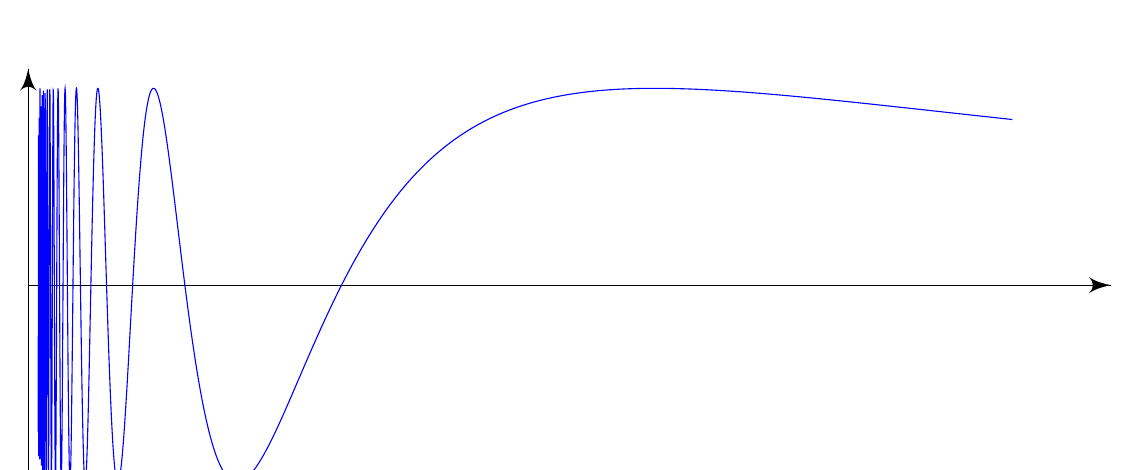
\begin{tikzpicture}[x=5cm, scale=2.5]
        \draw[->] (0,0) -- (1.1,0);
        \draw[->] (0,-1) -- (0,1.1);
      \draw[blue,domain=0.01:1,samples=5000] plot (\x, {sin((1/\x)r)});
    \end{tikzpicture}
  \end{center}

  \newpage
  \tableofcontents
  \newpage

  \section{Metric Spaces}\label{sec:metric-spaces}
  First we will begin with metric spaces.
  \begin{definition}[Metric space]
  Let $X$ be a non-empty set. A metric on $X$ is a function 
  $d \colon X \times X \to [0,\infty]$ such that for all $x,y,z \in X$,
  \end{definition}
  \begin{enumerate}
    \item[(1)] $d(x,y) = 0$ if and only if $x = y$;
    \item[(2)] $d(x,y) = d(y,x)$ (symmetry);
    \item[(3)] $d(x,z) \le d(x,y) + d(y,z)$ (triangle inequality);
  \end{enumerate}
  The pair $(X,d)$ is said to be a metric space.

  \subsection{Standard examples}

  \begin{example}
  Let $X$ be a non-empty set. Let $d \colon X \times X \to [0,\infty)$ be
  the function such that for $x,y \in X$,
  \[
    d(x,y) := \begin{cases}
      0, & x=y \\
      1, & x \neq y
    \end{cases}.
  \]
  The function $d$ is a metric and it is called the discrete metric on $X$.
  \end{example}
  \begin{example}
  Let $X = \R^n$ and define the function:
  \[
    d(x - y) := \abs{x - y},
  \]

  where $\abs{\cdot} \colon \R \to \R$ is the Eclidean norm function. 
  Then the pair $(X, d)$ forms a metric space.
  \end{example}

  \begin{example}
  Let $(X, N)$ be an arbitrary normed space and define the function:
  \[
    d(x - y) := N(x - y).
  \] 
  Then the pair $(X, d)$ forms a metric space.
  \end{example}

  \subsubsection{The \texorpdfstring{$L^p$}{} metric}

  \begin{example}
  The pair $(C\left([0,1]\right), d)$ such that $C([0,1])$ is the space of 
  all continuous functions on $[0,1]$ paired with the metric:
  \[
    d(f,g) = \int_{0}^{1}{\abs{f(x) - g(x)}\dx}
  \]
  is also a metric space. This metric is called the $L^1$ metric.
  \end{example}
  
  \begin{remark}
    In general, the $p$-metrics are induced by the $p$-norms, defined
    on $C\left([0,1]\right)$ for every $1 \le p < \infty$ as such:
    \[
      d(f,g) = \int_{0}^{1}{\abs{f(x) - g(x)}^p}\dx.
    \]
  \end{remark}
  Similarly we can define the $L^\infty$ space on $C\left([0,1]\right)$
  as in the following example.
  \begin{example}
  The pair $(C([0,1]), d)$ paired with the supremum metric:
  \[
    d(f,g) = \sup_{x \in [0,1]}{\abs{f(x) - g(x)}}
  \]
  is also metric space. This metric is called the $L^\infty$ metric.
  \end{example}
  
  \begin{example}
  Let $\Lambda$ be a nonempty set which will represent an alphabet.
  The set $\Lambda^{\N}$ represents all the sequences over that alphabet.
  The pair $(\Lambda^\N, d)$ with the metric $d$ defined on two sequences
  $\omega = (\omega_n)_{n=1}^{\infty}, \eta = (\eta_n)_{n=1}^{\infty}$
  as:
  \[
    d(\omega, \eta) = \begin{cases}
      2^{-\min\{n \geq 0 \mid \omega_n \neq \eta_n\}} & 
      \omega \neq \eta \\
      0 & \omega = \eta
    \end{cases}
  \]
  is also a metric space.
  \end{example}
  \begin{example}
    Another simple way to construct a metric space is by constructing it
    from another space. Let $(X,d)$ be a metric space and let $Y \subset X$.
    The pair $(Y,d_Y)$ where $d_Y$ is the metric $d$ constrained to $Y$
    is also a metric space, and it is called a metric subspace of $X$.
  \end{example}

  \subsection{Open sets}

  \begin{definition}[Open ball]
    Let $(X,d)$ be a metric space. For $x \in X$ and $r > 0$ write:
    \[
      B(x,r) := \set{y \in X \mid d(x,y) < r}.
    \]
    The set $B(x,r)$ is called the open ball in $X$ with center $x$
    and radius $r$.
  \end{definition}
  
  \begin{definition}[Open subset]
    A subset $U$ of a metric space $X$ is said to be open if for every
    $x \in X$ exists $r > 0$ such that $B(x,r) \subset X$.
  \end{definition}

  \begin{proposition}
    Every open ball in $X$ is an open subset of $X$.
  \end{proposition}
  \begin{proof}
    Let $B(x,r_x)$ be an open ball in $X$. Let $y \in B(x,r_x)$. Then for
    $r_y = r_x - d(x,y)$ we have that for every $z \in B(y,r_y)$ that
    \[
      d(x,z) \le d(x,y) + d(y,z) < d(x,y) + (r_x - d(x,y)) = r_x,
    \]
    which means that $B(y,r_y) \subset B(x,r_x)$ which completes the proof.
  \end{proof}

  \begin{proposition}[Properties of open subsets]
    The following properties are always satisfied:
    \begin{enumerate}
      \item[(1)] $\emptyset$ and $X$ are open;
      \item[(2)] A union of open sets remains open;
      \item[(3)] A finite intersection of open sets remains open;
    \end{enumerate}
  \end{proposition}
  These are the basic properties of open subsets, they can be verified
  directly from the definitions.

  \begin{proposition}
    A subset $U$ of $X$ is open if and only if it is a countable union of
    open balls.
  \end{proposition}
  \begin{proof}
    Let $U$ be a countable union of open balls, since every open ball is
    open, and a contable union of open subsets remains open, we get that
    $U$ is open in $X$.

    Let $U$ be an open subset of $X$. Then for every $x \in X$ exists
    $r_x > 0$ such that $B(x,r_x) \subset U$. We have that
    \[
      \bigcup_{x \in U} B(x,r_x) = U,
    \]
    which completes the proof.
  \end{proof}

  \begin{theorem}\label{thm:open-are-intervals}
    Every nonempty open subset of $\R$ is a countable union of disjoint
    open intervals.
  \end{theorem}
  Before we prove the following theorem, we need to prove a lemma.
  \begin{lemma}
    Let $\{I_\alpha\}_{\alpha \in A}$ be a family of open intervals of $\R$.
    Suppose that $\cap_{\alpha \in A} I_\alpha \neq \emptyset$, then 
    $\cap_{\alpha \in A} I_\alpha$ is an open interval.
  \end{lemma}
  \begin{proof}
    Let $x \in \cap_{\alpha \in A} I_\alpha$. For every $I_\alpha$ exists 
    $a_\alpha$, $b_\alpha$ such that $I_\alpha = (a_\alpha,b_\alpha)$.
    Denote
    \[
      a = \inf_{\alpha \in A} a_\alpha \quad \text{and} \quad
      b = \sup_{\alpha \in A} b_\alpha.
    \]
    We now clearly have that $\cup_{\alpha \in A} A_\alpha = (a,b)$, 
    which completes the proof.
  \end{proof}
  We will now prove \Cref{thm:open-are-intervals}.
  \begin{proof}
    Let $U \subset \R$ be open and nonempty.
    For any $x \in U$ let $I_x$ be the union of all open intervals $I \subset U$
    with $x \in I$.
    From the previous lemma we have that $I_x$ is an open interval for all
    $x \in U$. Consider the set
    \[
      \mathcal{E} := \set{I_x}{x \in U}.
    \]
    It is clear that $\cup_{I \in \mathcal E} I = U$.
    Notice that $I_x \neq I_y$ if and only if $I_x \cap I_y = \emptyset$.
    Since $\Q$ is dense in $\R$, for every $I \in \mathcal E$ exists 
    $q_I \in \Q$ such that $q \in I$. Since all the elements in $\mathcal E$
    are disjoint, we have that
    \[
      \abs{\mathcal E}=
      \abs{\set{q_I \mid I \in \mathcal E}} \le
      \abs{\Q} =
      \abs{\N},
    \]
    which completes the proof.
  \end{proof}
  
  \subsection{Sequences}

  \begin{definition}[Convergence]
    Let $\{x_n\}_{n \geq 1}$ be a sequence in $X$, and let $x \in X$.
    We say that $\{x_n\}_{n \geq 1}$ converges to $x$ and write
    \[
      x_n \taking{n \to \infty} x \quad \text{or} \quad \lim_{n \to \infty}
    \]
    if for all $\epsilon > 0$ there exists $N \geq 1$ such that
    $d(x_n,x) \le \epsilon$ for all $n \geq N$.
  \end{definition}

  \begin{proposition}[Uniqueness of the limit]
    Let $\{x_n\}_{n \geq 1}$ be a sequence in $X$ and $x, x' \in X$ such
    that $\{x_n\}_{n \geq 1} \taking{n \to \infty} x$ and
    $\{x_n\}_{n \geq 1} \taking{n \to \infty} x'$. Then $x = x'$.
  \end{proposition}
  \begin{proof}
    For all $n \geq 1$ we have that
    \[
      d(x,x') \le d(x,x_n) + d(x_n,x') < \epsilon.
    \]
    This shows that $d(x,x') \le 0$ and thus $d(x,x') = 0$ and $x = x'$
    as wanted.
  \end{proof}
  
  \subsection{Closed sets}

  \begin{definition}[Closed subset]
    We say that $F \subset X$ is a closed subset of $X$ if for every
    sequence $\{x_n\}_{n \geq 1} \subset F$ and $x \in X$ such that
    $\{x_n\}_{n \geq 1} \taking{n \to \infty} x$, we have that
    $x \in F$.
  \end{definition}
  \begin{proposition}
    Let $F$ be a subset of $X$. Then $F$ is closed if and only if 
    $X \setminus F$ is open.
  \end{proposition}
  \begin{proof}
    Suppose first that $F$ is not closed. Then exists $\{x_n\}_{n \geq 1}$
    and $x \in X$ such that $\{x_n\}_{n \geq 1}$ converges to $x$
    and $x \in X \setminus F$. Let $r > 0$, then we know that exists
    $N \geq 1$ such that for all $n > N$ we have
    \[
      d(x_n,x) < r \tand x_n \in X
    \]
    which shows that $X \setminus F$ is not open.

    Suppose next that $X \setminus F$ is not open. Then exists a sequence
    $x \in X$ such that for all $\frac{1}{n} > 0$ exists
    $x_n \in F$ such that $d(x,x_n) \le 1/n$. It follows that
    \[
      \{x_n\}_{n \geq 1} \taking{n \to \infty} x \tand
      x \in X \setminus F
    \]
    which shows that $F$ is not closed which completes the proof.
  \end{proof}

  \begin{proposition}[Properties of closed subsets]
    The following properties are always satisfied:
    \begin{enumerate}
      \item[(1)] $\emptyset$ and $X$ are closed;
      \item[(2)] An intersection of closed sets remains closed;
      \item[(3)] A finite union of closed sets remains closed;
    \end{enumerate}
  \end{proposition}
  These are the basic properties of closed subsets, they can be verified
  directly from the definitions.

  \begin{definition}[Closed ball]
    Let $(X,d)$ be a metric space. Let $x \in X$ and $r > 0$.
    We define
    \[
      \overline{B}(x,r) := \set{y \in X \mid d(x,y) \le B}. 
    \]
    The set $\overline{B}(x,r)$ is called the closed ball in $x$ with center
    $x$ and radius $r$.
  \end{definition}
  \begin{proposition}
    The set $\overline{B}(x,r)$ is a closed subset of $X$ for all $x \in X$
    and $r > 0$.
  \end{proposition}
  \begin{proof}
    It suffices to show that $X \setminus \overline B(x,r)$ is open.
  \end{proof}

  \subsubsection{The middle third Cantor set}

  \begin{example}[The middle third Cantor set]
    Set $C_0 := [0,1]$. Let $C_1$ be the set obtained by deleting the
    middle third of $C_0$, that is 
    $C_1 := \left[0,\frac 13\right] \cup \left[\frac 23,1\right]$.
    We can continue this process infinitely many times:
    \begin{align*}
      &C_0 := \intcc{0,1} \\
      &C_1 := \intcc{0,\frac 13} \cup \intcc{\frac 23,1} \\
      &C_2 := 
      \intcc{0, \frac 19} \cup
      \intcc{\frac 29, \frac 13} \cup
      \intcc{\frac 23, \frac 79} \cup
      \intcc{\frac 89, 1} \\
      &\phantom{C_k} \vdotswithin{:=}
    \end{align*}
    Since for every $n \in \N$ the set $\N$ is a finite union of closed
    sets, we have that $C_n$ are closed for all $n \in \N$. It then
    follows that the set $C := \cap_{n \in \N} C_n$ is also closed.
    The set $C$ is called the middle third Cantor set.
  \end{example}

  \subsection{Functions}

  \begin{definition}[Continuity]
    Let $f \colon X \to Y$ be a function between two metric spaces.
    We say that $f$ is continuous at $x \in X$ if for every $\{x_n\}_{n \geq 1}$
    \[
      \{x_n\}_{n \geq 1} \taking{n \to \infty} x \implies 
      \{f(x_n)\}_{n \geq 1} \taking{n \to \infty} f(x).
    \]
    We say that $f$ is continuous if it is continuous at $x$ for all
    $x \in X$.
  \end{definition}

  \begin{proposition}
    Let $f \colon X \to Y$ and $x \in X$ be given. Then $f$ is continuous
    at $x$ if and only if for every $\epsilon > 0$ there exists $\delta > 0$
    so that $f(B(x,\delta)) \subset B(f(x),\epsilon)$.
  \end{proposition}
  \begin{proof}
    To be added.
  \end{proof}

  \begin{proposition}
    A mapping $f \colon X \to Y$ is continuous if and only if $f^{-1}(U)$
    is open for every open $U \subset Y$.
  \end{proposition}
  \begin{proof}
    To be added.
  \end{proof}

  \newpage

  \section{Topological Spaces}\label{sec:topological-spaces}
  \begin{definition}[Topological space]
    Let $X$ be a nonempty set. A collection $\tau \subset P(X)$ is said to
    be a topology on $X$ if it satisfies the following properties,
    \begin{enumerate}
      \item[(1)] $X$, $\emptyset \in \tau$;
      \item[(2)] Any union of sets in $\tau$ is a set in $\tau$;
      \item[(3)] Any finite intersection of sets in $\tau$ is a set in $\tau$;
    \end{enumerate}
    The pair $(X,\tau)$ is said to be a topological space and $U \in \tau$
    an open set of $(X,\tau)$. An element $x \in X$ is said to be a point
    of $(X,\tau)$.
  \end{definition}

  \subsection{Standard examples}

  \begin{example}[Topology induced by metric]
    Every metric spaces can induce a topological space. Let $(X,d)$ be a
    metric space. Define
    \[
      \tau := \set{U \subset X \mid \forall x \in U \quad \exists \epsilon > 0
      \st B(x,\epsilon) \subset U}.
    \]
    It can be verified that $(X,\tau)$ is a topological space.
  \end{example}

  \begin{definition}[Metrizable space]
    We say that a topological space $(X,\tau)$ is metrizable, if exists a 
    metric $d$ on $X$, such that the topology that $d$ induces on $X$
    is equal to $\tau$.
  \end{definition}

  \begin{example}[Discrete topology]
    Let $X$ be a nonempty set and let $\tau := P(X)$. The topology $\tau$
    is called the discrete topology and the space $(X,\tau)$ is called the 
    discrete space. Is it metrizable?
  \end{example}

  \begin{example}[Trivial topology]
    Let $X$ be a nonempty set and let $\tau := \{\emptyset,X\}$. The topology 
    $\tau$ is called the trivial topology. Is it metrizable when $|X| = 1$?
    Is it metrizable when $|X| > 1$?
  \end{example}

  \begin{example}[Finite complement topology]
    Let $X$ be any infinite set and let 
    \[
      \tau := \set{A \subset X \mid \abs{X \setminus A} < \infty} \cup
      \{\emptyset\}.
    \]
    The topology $\tau$ is called the finite complement topology. Is it 
    metrizable?
  \end{example}
  
  \subsection{Continuous functions}

  \begin{definition}[Continuity]
    A mapping $f \colon X \to Y$ is said to be continuous if for every open
    set $U \subset Y$ the set $f^{-1}(U)$ is open.
  \end{definition}

  Notice that the definition for continuity in topological spaces is equivalent
  to the defintion we gave in metric spaces, under the topology induced by
  the metric.

  \begin{definition}[Neighbourhood]
    Given $x \in X$, an open $U \subset X$ containing $x$ is said to be a
    neighbourhood of $x$.
  \end{definition}

  \begin{definition}[Continuiuty at a point]
    A mapping $f \colon X \to Y$ is said to be continuous at $x$ if for 
    every neighbourhood $U$ of $f(x)$ there exists a neighbourhood $V$
    of $x$ such that $f(V) \subset U$.
  \end{definition}

  \begin{definition}[Open map]
    A mapping $f \colon X \to Y$ is said to be open if $f(U)$ is open in $Y$
    for every open $U \subset X$.
  \end{definition}
  
  \subsection{Homeomorphisms}

  \begin{definition}[Homeomorphism]
    A mapping $f \colon X \to Y$ is said to be a homeomorphism if it is
    injective, surjective, continuous and open. If there exists such an $f$, 
    then we say that $X$ and $Y$ are homeomorphic.
  \end{definition}

  \begin{proposition}
    Let $f \colon X \to Y$ be continuous. It follows that $f$ is a 
    homoemorphism if and only if it has a continuous inverse.
  \end{proposition}

  \begin{remark}
    We say that a property $P$ is a \emph{topological property} if for every
    two homeomorphic spaces $X$ and $Y$, then $P$ holds for $X$ if and only
    if it holds for $P$. The branch that deals with topological properties
    is called topology.
  \end{remark}

  \subsection{The subspace topology}

  \begin{definition}[Subspace topology]
    Let $(X,\tau_X)$ be a topological space and let $\emptyset \neq Y \subset 
    X$. Define
    \[
      \tau_Y = \set{U \cap Y \mid U \in \tau_X}
    \]
    We call $\tau_Y$ the subspace topology, induced by $\tau_X$ on $Y$.
  \end{definition}
  
  \subsubsection{Characteristic property of the subspace topology}

  \begin{theorem}
    \tt{Characteristic property of the subspace topology}
    Let $(X, \tau_X)$
    be a topological space, let $\emptyset \neq Y \subset X$, and write 
    $\tau_Y$ for the subspace topology on $Y$. Then $\tau_Y$ is the unique 
    topology on $Y$ which satisfies the following property. Let $Z$
    be a topological space and let $f \colon Z \to X$ be with 
    $f(Z) \subset Y$. Then $f$ is continuous as a map into $(X, \tau_X)$ if 
    and only if it is continuous as a map into $(Y, \tau_Y)$.
  \end{theorem}

  Throughout this section let $X$ be a fixed topological space.
  
  \subsection{Closed sets}

  \begin{definition}[Closed set]
    A subset $F$ of $X$ is said to be closed if $F^c = X \setminus F$ is open.
  \end{definition}

  \begin{proposition}[Properties of closed sets]
    The following properties are always satisfied:
    \begin{enumerate}
      \item[(1)] $X$, $\emptyset$ are closed;
      \item[(2)] Any intersection of closed sets is closed;
      \item[(3)] Any finite union of closed sets is closed;
    \end{enumerate}
  \end{proposition}

  \begin{definition}[Closure]
    Given $A \subset X$ we denote $\overline{A}$ to be the intersection of
    all $F \subset X$ such that $A \subset F$ and $F$ is closed. We call
    $\overline{A}$ the closure of $A$.
  \end{definition}

  \begin{remark}\label{rmk:closure}
    We can also define the closure of $A$ in an alternate way:
    \[
      \overline{A} = \set{x \in X \mid A \cap U \neq \emptyset \;\text{for each 
      neighbourhood $U$ of $x$}}.
    \]
    You may try to prove that both definitions are equivalent.
  \end{remark}

  \begin{definition}[Dense subset]
    A subset $A$ of $X$ is said to be dense in $X$ if $\overline{A} = X$.
  \end{definition}

  Using the second definition of closure we get that $A$ is dense in $X$
  if and only if $A \cap U \neq \emptyset$ for every nonempty $U \subset X$.

  \begin{definition}[Seperability]
    We say that $X$ is seperable if it has a countable dense subset.
  \end{definition}

  \begin{example}
    We know that $\Q$ is dense in $\R$. Since $\Q$ is countable, it follows
    that $\R$ is seperable.
  \end{example}

  \subsection{Isolated points and limit points}

  \begin{definition}[Isolated point]
    Let $A \subset X$. We say that $x$ is an isolated point of $A$ if exists
    $U$ open in $X$ such that $X \cap U = \{x\}$.
  \end{definition}

  This is exactly the same as saying that $x$ is an isolated point if and
  only if the singleton $\{x\}$ is open in the subspace topology.

  \begin{definition}[Limit point]
    Let $A \subset X$. We say that $x$ is a limit point of $A$ if for every
    neighourhood $U$ of $x$ there exists $a \in U \cap A$ with $a \neq x$.
    The set of all limit points of $A$ is called the derived set of $A$
    and is denoted by $D(A)$.
  \end{definition}

  \begin{example}
    Consider the set $A = \set{\frac{1}{n} \mid n \in \Z_{+}} \cup \{0\}$ as
    a subset of $\R$. Then $0$ is a limit point of $A$, and every
    other point in $A$ is an isolated point.
  \end{example}

  \begin{proposition}
    Let $A \subset X$ be given, then
    \begin{enumerate}
      \item $\overline{A} = A \cup D(A)$.
      \item $A$ is closed if and only if $D(A) \subset A$.
    \end{enumerate}
  \end{proposition}
  \begin{proof}
    Let $x \in X$. Suppose that $x \notin \overline A$. It follows that
    exists a neighbourhood $U$ of $x$ such that $U \cap A = \emptyset$.
    This implies that $x \notin D(A)$ and thus $x \notin A \cup D(A)$.

    Now suppose that $x \notin A \cup D(A)$. Since $x \notin D(A)$ exists
    a neighourhood $U$ of $x$ such that $U \cap A \setminus \{x\} = \emptyset$.
    Since $x \notin A$ we have $A = A \setminus \{x\}$ and thus
    $U \cap A = \emptyset$. This shows that $x \notin \overline A$ which
    completes the proof of the first part.

    For the second part, suppose that $D(A) \subset A$. This implies
    that $\overline A = A \cup D(A) = A$ which means that $A$ is closed.

    Next suppose that $A$ is closed. This implies that $\overline A = A$ and
    thus $A = A \cup D(A)$ which implies that $D(A) \subset A$ and completes
    the proof of the second part.
  \end{proof}

  \begin{corollary}
    Let $A \subset X$ be closed and write $I(A)$ for the set of all isolated
    points of $A$. Then $A$ is the disjoint union of $D(A)$ and $I(A)$.
  \end{corollary}
  \begin{proof}
    If $A$ is closed then $A = \overline A$ and then
    \[
      A = \overline A = A \cup D(A) = \left(A \setminus D(A)\right) \cup D(A) =
      I(A) \cup D(A).
    \]
    The last equality follows directly from the definitions and the fact
    that $I(A)$ and $D(A)$ are disjoint too.
  \end{proof}

  \subsection{The interior and boundary of a topological space}

  \begin{definition}[Interior]
    Let $A$ be a subset of $X$. The interior of $A$ is denoted by $\Int(A)$
    and is defined to be the union of all open subsets $U$ of $X$ so that 
    $U \subset A$. A point $x \in \Int(A)$ is said to be an interior point 
    of $A$ of a topological space.
  \end{definition}

  \begin{proposition}
    Let $A \subset X$ be given, then
    \begin{enumerate}
      \item $\Int{A} = X \setminus \overline{(X \setminus A)}$.
      \item $\Int(A)$ is open and contained in $A$.
      \item $A$ is open if and only if $A = \Int(A)$.
    \end{enumerate}
  \end{proposition}

  \begin{example}
    Considering $[a,b]$ as a subset of $\R$ we have $\Int([0,1]) = (0,1)$.
  \end{example}
  
  \begin{proposition}
    For $A \subset X$ we have
    \begin{enumerate}
      \item[(1)] $\Int(A) = X \setminus X \setminus \overline{(X \setminus A)}$;
      \item[(2)] $\Int(A)$ is open and contained in $A$;
      \item[(3)] $A$ is open if and only if $A = \Int(A)$;
    \end{enumerate}
  \end{proposition}

  \begin{definition}[Boundary]\label{dfn:boundary}
    Let $A \subset X$ be given. A point $x \in X$ is said to be a boundary
    point of $A$ if for every neighbourhood $U$ of $x$ we have 
    $U \cap A \neq \emptyset$ and $U \cap (X \setminus A) \neq \emptyset$.
    The set of all boundary points of $A$ is called the boundary of $A$ and 
    is denoted by $\partial A$.
  \end{definition}

  \begin{example}
    Considering $[a,b)$ as a subset of $\R$ we have $\partial A = \{a,b\}$.
  \end{example}

  \begin{proposition}
    For $A \subset X$ we have 
    $\partial A = \overline{A} \cap \overline{X \setminus A}$ and in 
    particular $\partial A$ is closed.
  \end{proposition}
  \begin{proof}
    The equality follows directly from \Cref{dfn:boundary} and
    \Cref{rmk:closure}. We have that $\partial A$ is closed as it
    it an intersection of two closed sets.
  \end{proof}

  \begin{proposition}
    Let $A \subset X$ be given, then $\overline A$ is the disjoint union of 
    $\Int(A)$ and $\partial A$.
  \end{proposition}
  
  \subsection{Open bases}

  \begin{definition}[Open base]
    A family $\mathcal{B}$ of subsets of $X$ is said to be an open base
    for $X$ if for each open $U \subset X$ and $x \in U$ exists 
    $B \in \mathcal{B}$ such that $x \in B \subset U$.
  \end{definition}

  \begin{remark}
    It is easy to see that a family $\mathcal{B}$ of open subsets of $X$ is an 
    open base for $X$ if and only if each open $U \subset X$ is a union of 
    elements of $\mathcal{B}$.
  \end{remark}

  \begin{proposition}\label{prp:base-continuity}
    Let $Y$ be a topological space, let $\mathcal B$ be an open base for $Y$, 
    and let $f \colon X \to Y$. 
    Suppose that $f^{-1}(B)$ is open for all $B \in \mathcal B$,
    then $f$ is continuous.
  \end{proposition}

  \subsubsection{Countability}

  \begin{definition}[Second countability]
    We say that $X$ is second countable, or that it satisfies the second
    axiom of countability, if it has a countable open base.
  \end{definition}

  \begin{proposition}
    Suppose that $X$ is second countable, then $X$ is separable.
  \end{proposition}

  \begin{proof}
    Let $\mathcal{B}$ be a countable open base for $X$. We have that 
    $\mathcal{B} \setminus \{\emptyset\}$ is also an open base. Choose
    an arbitrary $x_B \in B$ for each $B \in \mathcal{B}$. Since 
    $\mathcal{B}$ is countable $\{x_B\}_{B \in \mathcal{B}}$ is also 
    countable. Let $U$ be open in $X$. By defintion of an open base exists 
    $B \in \mathcal{B}$ such that $x_B \in B$ and $B \subset U$ so 
    $x_B \in U$. This shows that $\{x_B\}_{B \in \mathcal{B}}$ is dense
    in $X$ and thus $X$ is seperable.
  \end{proof}

  \begin{remark}
    In metric spaces, the property of being seperable and second countable
    is equivalent. If we denote $(X,d)$ the metric space and $A$ the 
    countable dense set, then
    \[
      \mathcal{B} = \set{B(a,q) \mid a \in A \text{ and } q \in \Q \cap 
      (0,\infty)}
    \]
    will form the desired countable open base for $X$.
  \end{remark}

  \begin{example}
    A classic example of a topological space that is seperable but not
    second countable is the Sorgenfrey line, also known as the lower
    limit topology, which we will discuss later.
  \end{example}

  \begin{theorem}
    \tt{Lindelöf’s Theorem} Suppose that $X$ is second countable. Let
    $\{U_i\}_{i \in I}$ be a family of open subsets of $X$. Then there
    exists a countable $I_0 \subset I$ so that 
    $\cup_{i \in I_{0}}{U_i} = \cup_{i \in I}{U_i}$
  \end{theorem}
  \begin{proof}
    Let $\mathcal{B}$ be a countable open base for $X$. Set,
    \[
      \mathcal{B}_0 = \set{B \in \mathcal{B} \mid B \subset U_i
      \text{ for some } i \in I}
    \]
    For each $B \in \mathcal{B}_0$ choose an arbitrary $i_B \in I$ such
    that $B \subset U_{i_B}$. Set $I_0 = \set{i_B \mid B \in \mathcal{B}_0}$.
    Since $\mathcal{B}$ is countable, $I_0$ is also countable. It remains
    to show that $\cup_{i \in I_{0}}{U_i} = \cup_{i \in I}{U_i}$. Let
    $x \in \cup_{i \in I}{U_i}$ then exists some $j$ such that $x \in U_j$
    since $\mathcal{B}$ is an open base exists $B \subset U_j$ such that
    $x \in B$. By definition we see that $B \in \mathcal{B}_0$, thus
    $i_B \in I_0$ and then:
    \[
      x \in B \subset U_{i_B} \subset \cup_{i \in I_{0}}{U_i}
    \]
    The other side of the inclusion is obvious which concludes the proof.
  \end{proof}

  \begin{corollary}
    Suppose that $X$ is second countable and that $\mathcal{B}$ is an open
    base for $X$. Then exists a countable $\mathcal{B}_0 \subset \mathcal{B}$ 
    which is also an open base for $X$.
  \end{corollary}
  \begin{proof}
    Let $\mathcal{E}$ be a countable open base for $X$. Since $\mathcal{B}$
    is an open base, for each $E \in \mathcal{E}$ exists 
    $\mathcal{B}_E \subset \mathcal{B}$ such that 
    $E = \cup_{B \in \mathcal{B}_E} B$. From Lindel\"of's theorem
    we get that exists a countable $\mathcal{B}^0_E \subset \mathcal{B}_E$
    such that $U_{B \in \mathcal{B}^0_E} = \cup_{i \in \mathcal{B}_E}{U_i}$.
    Now set $\mathcal{B}_0 = \cup_{E \in \mathcal{E}}{\mathcal{B}^0_E}$.
    It is countable as a countable union of countable sets. Moreover,
    since $\mathcal{E}$ is an open base, and since each $E \in \mathcal{E}$
    is a union of elements from $\mathcal{B}_0$, it is clear that
    $\mathcal{B}_0$ is also an open base for $X$ which completes the proof.
  \end{proof}

  \begin{definition}[Open base at a point]
    Let $x \in X$. A class of neighbourhoods $B_x$ of $x$ is called an open
    base at $x$ if for every neighbourhood $U$ of $x$ exists $B \in B_x$
    such that $B_x \subset U$.
  \end{definition}

  \begin{definition}[First countability]
    We say that $X$ is first countable, or that it satisfies the first
    axiom of countability, if for each $x \in X$ there exists a countable 
    open base at $x$.
  \end{definition}

  \begin{remark}
    It is clear that if $X$ is second countable, it is also first countable.
  \end{remark}

  \begin{example}
    Let $(X, d)$ be a metric space. For each $x \in X$ the collection
    \[
      \set{B\del{x, 1/n} \mid n \geq 1}
    \]
    is a countable open base at $x$. 
    Thus every metric space is first countable.
  \end{example}

  \subsection{Open subbases}

  \begin{definition}[Open subbase]
    Let $X$ be a topological space. A family $\mathcal{S}$ of open subsets 
    of $X$ is said to be an open subbase for $X$ if the collection of all 
    finite intersections of elements of $\mathcal{S}$ forms an open base 
    for $X$.
  \end{definition}

  \begin{proposition}
    Let $X$ and $Y$ be topological spaces, let $\mathcal{S}$ be an open
    subbase for $Y$. Then if $f^{-1}(S)$ is open for each $S \in \mathcal{S}$
    then $f$ is continuous.
  \end{proposition}
  \begin{proof}
    For $S_1,\dots,S_n$ we have that 
    $f^{-1}(\cap_{i=1}^{n} S_i) = \cap_{i=1}^{n} f^{-1}(S_i)$.
    Therefore, for any finite intersection of elements of $\mathcal S$,
    in other words, for any element $U$ of some open case $\mathcal B$
    we have $f^{-1}(U)$ is open. The result now follows directly by 
    \Cref{prp:base-continuity}.
  \end{proof}

  The above proposition shows how convenient working with subbases can be.
  The following will show how to easily generate topologies using the notion.

  \begin{proposition}
    Let $X$ be an aribitrary nonempty set, 
    and let $\mathcal{S} \subset P(X)$. Set,
    \[
      \mathcal{B} := \set{\cap_{i=1}^{n}{S_i} \mid n \geq 0 \textnormal{ and }
      S_1,\dots,S_n \in \mathcal{S}}
    \]
    And,
    \[
      \tau := \set{U \subset X \mid \forall x \in U \quad \exists B \in 
      \mathcal{B} \st x \in B \subset U}
    \]
    Then $\tau$ is a topology on $X$, $\mathcal{B}$ is an open base for 
    $\tau$ and $\mathcal{S}$ is an open subbase for it.
  \end{proposition}

  Sometimes we need to compare topologies. Let $\mathcal{T}(X)$ be the set of
  all topologies on a set $X$.

  \begin{definition}[Comparison of topologies]
    Let $\tau_1,\tau_2 \in \mathcal{T}(X)$. We say that $\tau_1$ is weaker
    than $\tau_2$, or that $\tau_2$ is stronger than $\tau_1$ if 
    $\tau_1 \subset \tau_2$.
  \end{definition}

  For a simple reality check, notice that every topology is weaker than the
  discrete topology and stronger than the discrete topology. Also, the
  pair $(\mathcal{T}(X), \subset)$ form a partially ordered set.

  \begin{proposition}
    Let $\mathcal T_0 \subset \mathcal T(X)$ be nonempty. Then $\mathcal T_0$
    has a supremum and an infimum in $\mathcal T(X)$
  \end{proposition}
  \begin{proof}
    This is more of a sketch proof, but it can be verified that taking the
    intersection of all $\tau \in \mathcal T_0$ gives the infimum of 
    $\mathcal T_0$, and that taking the intersection of all 
    $\tau \in \mathcal T(X)$ that are stronger than every 
    $\tau \in \mathcal T_0$ gives the supremum of $\mathcal T_0$.
  \end{proof}

  \begin{remark}
    It can also be seen that the supremum of $\mathcal T_0$ is exactly the
    topology generated by $\cup_{\tau \in \mathcal T_0} \tau$.
  \end{remark}

  \subsection{Topology generated by functions}

  \begin{definition}[Topology generated by functions]
    Let $\{Y_i\}_{i \in I}$ be a family of topological spaces. For each
    $i \in I$ let $f_i \colon X \to Y_i$. Write $\mathcal{T}_0 \subset 
    \mathcal{T}(X)$ for the set of all topologies with respect to which all
    $\{f_i\}_{i \in I}$ are continuous. The greatest lower bound of 
    $\mathcal{T}_0$ is called the weak topology generated by 
    $\{f_i\}_{i \in I}$.
  \end{definition}

  \begin{remark}
  It is easy to verify that $\tau = \cap_{\tau_0 \in \mathcal{T}_0}{\tau_0}$
  and also that $\tau$ is generated by the set
  \[
    S = \set{f_i^{-1}(U) \mid i \in I \text{ and $U$ is open in $Y_i$}}
  \]
  \end{remark}

  \begin{example}
    Let $Y$ be a topological space, let $Z$ be a nonempty subset of $Y$,
    and let $f \colon Z \to Y$ be the inclusion map, that is $f(z) = z$ 
    for $z \in Z$. It is easy to show that the weak topology generated by $f$ 
    is equal to the subspace topology induced by $Y$ on $Z$.
  \end{example}

  \subsection{The product topology}

  \begin{definition}[Product topology]
    The product topology on a cartesian product of topological spaces
    $\prod_{i \in I} X_i$ is defined to be the weak topology generated by
    the projections $\{\pi_i\}_{i \in I}$. Equipped with the product
    topology, the space $X$ is called the product space of the spaces
    $\{X_i\}_{i \in I}$.
  \end{definition}

  This definition is a bit abstract, but we can give a more concrete 
  definition by setting,
  \[
    \mathcal{S} = \set{\prod_{i \in I}{U_i} \mid \exists j \in I \st 
    \text{ $U_i = X_i$ for $i \in I \setminus \{j\}$ and $U_j$ is open in
    $X_j$}}.
  \]
  Now the product topology on $X$ is equal to the topology on $X$ generated
  by $\mathcal{S}$ as a subbase. From this we can also deduce that
  {\small
  \[
    \mathcal{B} = \set{\prod_{i \in I}U_i \mid \text{Exists a finite
    $I_0 \subset I$ \st $U_i = X_i$ for $i \in I \setminus I_0$ and
    $U_i$ is open in $X_i$ for $i \in I_0$}}
  \]
  }
  is an open base for the product topology.

  \begin{definition}[Euclidean topology]
    The Euclidean topology is the natural topology induced on $n$-dimensional 
    Euclidean space $\R^n$ by the Euclidean metric. The open balls, and
    the open boxes both form open bases for this topology.
  \end{definition}

  \begin{example}
    Considering the space $\R^n$ for a finite natural $n$, the Euclidean
    topology on it is equal to the product topology of the product of
    $\prod_{i=1}^{n} \R$ where each copy of $\R$ has been endowed with
    the standard topology. This is not true in the case of $\R^J$ where
    $J$ is an infinite set.
  \end{example}

  \begin{proposition}
    \tt{Characteristic property of the product topology}
    The product topology is the unique topology on $X$ which satisfies the 
    following property. Let $Y$ be a topological space and let 
    $f \colon Y \to X$. Then $f$ is continuous if and only if 
    $\pi_i \circ f$ is continuous for each $i \in I$.
  \end{proposition}

  \begin{definition}[The function algebras]
    Let $X$ be a topological space. We write $C(X)$ for the collection of 
    all continuous functions from $X$ to $\R$. We denote by $C_b(X)$ the set 
    of all bounded elements of $C(X)$. It has the a natural norm defined on
    it, the supremum norm.
  \end{definition}

  More about algebras in \Cref{sec:the-AA-theorem}.

  \newpage

  \section{Complete Metric Spaces}\label{sec:complete-metric-spaces}
  Let $(X,d)$ be a fixed metric space.

  \subsection{Definitions}

  \begin{definition}[Cauchy sequence]
    We say that a sequence $\{a_n\}_{n \geq 1} \subset X$ is a Cauchy
    sequence if for all $\epsilon > 0$ exists $N \geq 1$ such that 
    $d(x_n,x_m) < \epsilon$ for all $n,m > N$.
  \end{definition}

  It is easy to verify that all Cauhcy sequences converge, but the converse
  is not always true. This leads us to formulate the following notion.

  \begin{definition}[Complete space]
    We say that the metric space $(X,d)$ is complete if every Cauchy
    sequence $\{a_n\}_{n \geq 1} \subset X$ converges to some $x \in X$.
  \end{definition}

  \begin{remark}
    Consider the set $(-1,1)$ with the topology induced by $\R$. It is
    clear that the sequence $1 - \frac{1}{n}$ is a cauchy sequence, but
    it's limit is $1 \notin (-1,1)$ and thus the space is not complete.
    However, there is a homeomorphism $x \mapsto \tan(\pi x/2)$ between
    $(-1,1)$ and $\R$, and $\R$ is complete which shows that completeness
    is not a topological property.
  \end{remark}

  \subsection{Examples of complete metric spaces}

  \subsubsection{Banach spaces}

  \begin{definition}[Banach space]
    A complete normed space is said to be a Banach space.
  \end{definition}

  \begin{example}
    Let $X$ be a topological space. We will show that $C_b(X)$ is a Banach
    space with respect to the metric induced by the supremum norm 
    $\norm{\cdot}_{\infty}$. Let $\{f_n\}_{n \geq 1}$ be a Cauchy sequence
    in $C_b(X)$. Then, by the definition of the supremum norm we have that
    for any $x \in X$ that the sequence $\{f_n(x)\}_{n \geq 1}$ is a Cauchy
    sequence in $\R$, and since $\R$ is complete it also has a limit.
    Thus, exists $f \colon Y \to \R$ such that 
    $\{f_n(x)\}_{n \geq 1} \taking{n \to \infty} f$ pointwise.
    Now, we see that
    \begin{align*}
      \abs{f(x) - f_n(x)} &\le
      \limsup_{m \to \infty}(\abs{f(x) - f_m(x)} + \abs{f_m(x) - f_n(x)}) \\
      &\le \limsup_{m \to \infty} \norm{f(x) - f_n(x)}_{\infty}.
    \end{align*}
    Thus, $f_n \taking{n \to \infty} f$ uniformly,
    which implies that $f \in C_b(X)$. We have also shown that
    $f_n \taking{n \to \infty} f$ uniformly with respect to $\norm{\cdot}$
    which completes the theorem.
  \end{example}

  \subsubsection{Subspace of a complete metric space}

  \begin{proposition}
    Suppose that $X$ is complete and let $Y$ be a nonempty subset of $X$. 
    Then $Y$ is complete (with respect to the metric induced by $X$) if and 
    only if $Y$ is closed in $X$.
  \end{proposition}
  \begin{proof}
    Suppose first that $Y$ is closed. Let $\{y_n\}_{n \geq 1}$ be a Cauchy
    sequence in $Y$. Then since $X$ is complete there exists a limit $y \in X$
    to $\{y_n\}_{n \geq 1}$. Since $Y$ is closed we have that $y \in Y$
    which shows that $Y$ is complete.

    Suppose next that $Y$ is complete. Let $\{y_n\}_{n \geq 1}$ be a sequence
    in $Y$ that converges to some $x \in X$. Since it converges in $X$,
    it must be a Cauchy sequence. By the definition of the subspace metric
    we have that the sequence is also Chauchy in $Y$. Since $Y$ is complete
    $\{y_n\}_{n \geq 1}$ must also have a limit in $Y$. From the uniqueness
    of the limit we have that $x \in Y$. It follows that $Y$ is closed.
  \end{proof}

  \subsection{Cantor’s intersection lemma}
  
  \begin{definition}[Diameter]
    Given a nonempty subset $A$ of $X$ we write
    \[
      \diam(A) := \set{d(x_1,x_2) \mid x_1,x_2 \in X}.
    \]
    We call the number $\diam(A)$ the diameter of $A$.
  \end{definition}
  
  The following lemma demonstrates the usefulness of the completeness property.
  
  \begin{lemma}
    \tt{Cantor’s intersection lemma for complete metric spaces}
    Let $F_1,F_2,\dots$ be nonempty closed subsets of $X$. Suppose that
    \begin{itemize}
      \item $X$ is complete;
      \item $F_{n+1} \subset F_{n}$ for all $n \geq 1$;
      \item $\diam(F_n) \to 0$ as $n \to \infty$.
    \end{itemize}
    Then $\cap_{n \geq 1}{F_n} = \{x\}$ for some $x \in X$.
  \end{lemma}
  \begin{proof}
    For each $n \geq 1$ choose $x_n \in F_n$. For each $n \geq m \geq 1$
    we have that $x_n,x_m \in F_n$ and thus $d(x_n,x_m) \le \diam(F_n)$.
    Since $\diam(F_n) \to 0$ we have that $\{x_n\}_{n \geq 1}$ is a Cauchy
    sequence in $X$. Since $X$ is complete exists $x \in X$ such that 
    $x_n \to x$ as $n \to \infty$. For each $n \geq 1$ we have that 
    $\{x_m\}_{m \geq n} \subset F_n$ and since each $F_n$ is closed, we
    have that $x \in F_n$. Thus $x \in \cap_{n \geq 1}{F_n}$ and in 
    particular $\cap_{n \geq 1}{F_n} \neq \emptyset$. Let 
    $x,y \in \cap_{n \geq 1}{F_n}$. We have that $d(x,y) \le \diam(F_n)$
    for each $n \geq 1$. Since $\diam(F_n) \to 0$ as $n \to \infty$ we
    have that $d(x,y) = 0$ and thus $x=y$. This implies that
    $\cap_{n \geq 1}{F_n} = \{x\}$ which completes the proof.
  \end{proof}
  
  \subsection{The completion theorem}

  \begin{definition}[Isometry]
    Let $(X,d_X)$ and $(Y,d_Y)$ be metric spaces. A map $f \colon X \to Y$ 
    is said to be an isometry if $d_X(x_1,x_2) = d_Y(f(x_1),f(x_2))$ for all 
    $x_1,x_2 \in X$. We say that $X$ and $Y$ are isometric if there exists 
    an isometry from $X$ onto $Y$.
  \end{definition}
  
  \begin{remark}
    Every isomorphism is continuous and injective. A surjective isomorphism
    is thus a homeomorphism.
  \end{remark}
  
  \begin{theorem}
    \tt{The completion theorem for metric spaces}
    Let $X$ be a metric space. Then there exists a complete metric space
    $\overline{X}$ and an isometry $f \colon X \to \overline{X}$ such that 
    $f(X)$ is dense in $\overline{X}$. Moreover, if $Y$ is another complete 
    metric space such that exists an isometry $g \colon X \to Y$ such that
    $g(X)$ is dense in $Y$ then there exists a surjective isometry
    $h \colon \overline{X} \to Y$ so that $g = h \circ f$.
  \end{theorem}
  \begin{proof}
    To be added.
  \end{proof}

  \begin{remark}
    The space $\overline{X}$ is called the completion of $X$. As the theorem
    states it is unique up isometry.
  \end{remark}
  
  \begin{definition}[Uniform continuity]
    A mapping $f \colon X \to Y$ is said to be uniformly continuous if for
    every $\epsilon > 0$ there exists $\delta > 0$ so that 
    $d_Y(f(x_1),f(x_2)) < \epsilon$ for all $x_1,x_2 \in X$ with 
    $d_X(x_1,x_2) < \delta$.
  \end{definition}
  
  \begin{proposition}
    Let $A \subset X$, let $f \colon X \to Y$ be uniformly continuous.
    Then there exists a unique $\overline{f} \colon \overline{X} \to Y$ 
    which extends $Y$ such that $\overline{f}$ is also continuous.
  
  \end{proposition}
  
  \subsection{Baire's theorem}
  
  \begin{definition}[Nowhere dense subset]
    A subset $A$ of $X$ is said to be nowhere dense if 
    $\Int\left(\overline A\right) = \emptyset$.
  \end{definition}
  
  \begin{remark}
    Note that a closed subset $A \subset X$ is nowhere dense if and only if 
    $\Int(A) = \emptyset$.
  \end{remark}
  
  \begin{example}
    Let $W$ be a linear subspace of $\R^d$ with $\dim W < d$. We will show
    that $W$ is nowhere dense. Let $\ip{\cdot}{\cdot}$ be the standard
    inner product on $\R^d$. We notice that for every $v \in \R^d$ the
    map $x \mapsto \ip{x}{v}$ is continuous. Thus the set 
    $\set{x \in \R^d \mid f(x) = 0}$ is closed in $\R^d$ as the preimage of the
    closed set $\{0\}$. From this and from the fact that:
    \[
      W = (W^{\perp})^{\perp} = 
      \cap_{u \in W^{\perp}}{\set{x \in \R^d \mid \ip{x}{u} = 0}},
    \]
    it follows that $W$ is closed in $\R^d$. Moreover, for every $w \in W$,
    $0 \neq u \in W^{\perp}$ and $\epsilon > 0$ we have that 
    $w+u\epsilon \notin W$. Since $W^{\perp} \neq \emptyset$ that means that
    $\Int(W) = \emptyset$, which shows that $W$ is nowhere dense.
  \end{example}
  
  \begin{definition}[First category]
    A subset $E$ of $X$ is said to be of the first category if there exist
    nowhere dense subsets $A_1,A_2,\dots \subset X$ so that 
    $E = \cup_{n \geq 1}{A_n}$. A subset of $X$ which is not of the first 
    category is said to be of the second category.
  \end{definition}

  \begin{theorem}
    \tt{The Baire category theorem}
    Suppose that $X$ is complete, and let $E \subset X$ be of the first
    category. Then $\Int(E) = \emptyset$.
  \end{theorem}
  \begin{proof}
    It suffices to prove that exists $x_0 \in X$ and $\epsilon_0 > 0$ such
    that $B(x_0,\epsilon) \setminus E \neq \emptyset$. Since $E$ is of
    the first category, there exist closed subsets $F_1,F_2,\dots$ such that
    $E \subset \cup_{n \geq 1}{F_n}$ and $\Int(F_n) = \emptyset$ for each
    $n \geq 1$. We are going to construct sequences 
    $\{e_n\}_{n \geq 1} \subset (0,\infty)$ such that 
    $\epsilon_n < \frac{1}{n}$ and $\overline{B}(x_n,\epsilon_n) \subset
    B(x_{n-1},\epsilon_{n-1}) \setminus \cup_{k=1}^{n}{F_k}$. 
    
    Let $n \geq 1$ and assume that we already constructed the sequences
    for $1 \le k \le n-1$. From 
    $B(x_{n-1},\epsilon_{n-1}) \cap (\cup_{k=1}^{n-1}{F_n}) = \emptyset$ 
    it follows that 	
    $V:=B(x_{n-1},\epsilon_{n-1}) \setminus \cup_{k=1}^{n-1}{F_n} 
    \neq \emptyset$. From this, and since $V$ is open and 
    $\Int(F_n) = \emptyset$ we get that $V \setminus F_n \neq \emptyset$.
    Since $V \setminus F_n$ is nonempty and open we get that there exists
    $x_n \in X$ and $0 < \epsilon_n < \frac{1}{n}$ such that
    $\overline{B}(x_n,\epsilon_n) \subset V \setminus F_n = 
    B(x_{n-1},\epsilon_{n-1}) \setminus \cup_{k=1}^{n}{F_k}$.
    This completes the inductive construction.
    
    From Cantor's intersection lemma it now follows that
    $\cap_{n \geq 1}{\overline{B}(x_n,\epsilon_n)} = \{x\}$ for some
    $x \in X$. For every $n \geq 1$ we have 
    $x \in \overline{B}(x_n,\epsilon_n) \subset 
    B(x_{n-1},\epsilon_{n-1}) \setminus \cup_{k=1}^{n}{F_k}$. This
    shows that:
    \[
      x \in B(x_{0},\epsilon_{0}) \setminus \cup_{k=1}^{\infty}{F_k}
      \subset B(x_0,\epsilon_0) \setminus E,
    \]
    which completes the proof of the theorem.
  \end{proof}
   
  The following is an immediate corollary from Baire's theorem.
  
  \begin{corollary}
    Suppose that $X$ is complete. Then $X$ is of the second category as a
    subset of itself. Consequently, if $F_1,F_2,\dots$ are closed subsets 
    of $X$ with $X = \cup_{n \geq 1}{F_n}$, then $\Int(F_n) \neq \emptyset$ 
    for some $n \geq 1$.
  \end{corollary}
  
  Here's another useful corollary of Baire's theorem.
  
  \begin{corollary}
    Suppose that $X$ is complete. Let $U_1,U_2,\dots$ be open subsets of $X$.
    Suppose that $U_n$ is dense in $X$ for all $n \geq 1$. Then 
    $\cap_{n \geq 1}{U_n}$ is also dense in $X$.
  \end{corollary}
  \begin{proof}
    For $n \geq 1$ set $F_n := X \setminus U_n$. Since $U_n$ is dense in $X$
    for all $n \geq 1$ it follows that $F_n$ is nowhere dense in $X$ for
    all $n \geq 1$. Let $V \subset X$ be open. Then by Baire's category
    theorem we have that the interior of $\cup_{n=1}^{\infty} F_n$ is
    empty and thus
    \[
      \emptyset \neq 
      V \setminus \cup_{n=1}^{\infty} F_n =
      V \cap \cap_{n \geq 1}{U_n}
    \]
    which completes the proof.
  \end{proof}
  
  \begin{definition}[The sets $G_\delta$ and $F_\sigma$]
    Let $Y$ be a topological space. A countable intersection of open
    subsets of $Y$ is called a $G_\delta$ set. A countable union of closed 		
    subsets of $Y$ is called an $F_\sigma$ set.
  \end{definition}

  \begin{definition}[Liouville number]
    An irrational real number $x$ is said to be a Liouville number if
    for every integer $n \geq 1$ there exist integers $p$ and $q \geq 2$ 
    so that $\abs{x - \frac{p}{q}} < \frac{1}{q^n}$.
  \end{definition}

  \begin{example}
    The number $\sum_{k \geq 1}{\frac{1}{10^{k!}}}$ is called Liouville’s 
    constant. It is not difficult to show that it is a Liouville number.
  \end{example}

  \begin{proposition}
    Write $L$ for the set of Liouville numbers. Then $L$ is a dense
    $G_\delta$ subset of $\R$.
  \end{proposition}
  \begin{proof}
    For every $n \geq 1$ set
    \[
      V_n := \bigcup_{q=2}^{\infty} \bigcup_{p \in \Z}
      \left(\frac{p}{q} - \frac{1}{q^n},\frac{p}{q} + \frac{1}{q^n}\right).
    \]
    Note that $\Q \subset V_n$ which means $V_n$ is dense in $\R$. For each
    $r \in \Q$ denote $U_r = \R \setminus \{r\}$. It follows directly from
    the definition of Liouville numbers that:
    \[
      L = \left(\bigcap_{n=1}^{\infty}{V_n}\right) \cap
        \left(\bigcap_{r \in \Q}{U_r}\right)
    \]
    Now since that sets $\{V_n\}_{n=1}^{\infty}$ and $\{U_r\}_{r \in \Q}$
    are all open and dense, and since $\Q$ is countable, it follows from
    the previous corollary that $L$ is a dense $G_\delta$ subset of $\R$.
    This completes the proof.
  \end{proof}

  \subsection{The Banach fixed-point theorem}

  \begin{definition}[Contraction]
    A mapping $f \colon X \to X$ is called a contraction of $X$ if there 
    exists $c \in [0, 1)$ so that $d(f(x),f(y)) \le cd(x,y)$ for all 
    $x,y \in X$.
  \end{definition}

  \begin{theorem}
    \tt{The Banach fixed-point theorem}
    Suppose that $X$ is complete
    and let $f \colon X \to X$ be a contraction. Then $f$ has a unique fixed 
    point. That is, there exists a unique $x \in X$ so that $f(x) = x$.
  \end{theorem}
  \begin{proof}
    First we show that $f$ has a fixed point. Choose an arbirary $x_0 \in X$
    and define a sequence $\{x_n\}_{n \geq 0}$ by setting
    $x_n := f(x_{n-1})$ for $n \geq 1$. It is easy to show by induction
    that:
    \[
      d(x_{n+1},x_{n}) \le c^n d(x_1,x_0)
    \]
    Now we will show that $\{x_n\}_{n \geq 1}$ is a Cauchy sequence.
    Let $\epsilon > 0$. Choose $N \geq 1$ such that
    $c^N d(x_0,x_1) (1-c)^{-1} < \epsilon$. For $n \geq m \geq N$,
    \begin{align*}
      d(x_n,x_m) \le 
      \sum_{k=m}^{n-1}{d(x_{k},x_{k+1})} &\le 
      \sum_{k=m}^{n-1}{c^k d(x_{0},x_{1})} \\ &\le
      c^m d(x_0,x_1) \sum_{k=1}^{\infty}{c^k} =
      \frac{c^m d(x_0,x_1)}{1-c} < \epsilon
    \end{align*}
    which shows that $\{x_n\}_{n \geq 1}$ is Cauchy. Since $X$ is complete
    exists $x \in X$ such that $\{x_n\}_{n \geq 1} \to x$ as $n \to \infty$.
    Since $f$ is a contraction it is continuous. We get:
    \[
      x = \lim_{n\to\infty}{x_n} = \lim_{n \to \infty}{f(x_{n-1})} = f(x),
    \]
    which shows that $f$ has a fixed point.
    
    Next we show uniqueness. Suppose there were $y \in X$ another fixed
    point of $f$. Then
    \[
      d(x,y) = d(f(x),f(y)) \le cd(x,y)
    \]
    Thus we have $(1-c)d(x,y) \le 0$. This is only possible if $d(x,y)=0$
    thus $x=y$ which completes the proof.
  \end{proof}

  Notice that the proof of the theorem also gives an explicit way to 
  approximate the fixed point of $f$.

  \subsection{A glimpse of Picard’s theorem}

  The following is a simplified version of the Picard–Lindelöf theorem 
  regarding the existence and uniqueness of solutions for ordinary 
  differential equations, which is also sometimes called the existence and 
  uniqueness theorem.

  For $\epsilon > 0$ we set $I_\epsilon := [-\epsilon, \epsilon]$.

  \begin{theorem}
    \tt{Picard's theorem}
    Let $F \colon I_1 \times I_1 \to \R$ be continuous. Suppose that there 
    exists $K > 0$ so that $\abs{F(t,x) - F(t,y)} \le K\abs{x - y}$ for all 
    $t, x, y \in I_1$. Then there exists $\epsilon > 0$ for which there 
    exists a unique $f \colon I_{\epsilon} \to I_{1}$ so that,
    \begin{itemize}
      \item $f$ is differentiable on $I_{\epsilon}$;
      \item $f(0)=0$
      \item $f'(t) = F(t,f(t))$ for $t \in I_{\epsilon}$
    \end{itemize}
  \end{theorem}
  \begin{example}
    Suppose that $F(t,x) = 1 + x^2$. Since $\tan(0) = 0$, and on 
    $\left(- \frac{\pi}{2}, \frac{\pi}{2}\right)$ we have
    \[
      [\tan(x)]' = \frac{1}{\cos^2(x)} = 1 + \tan^2(x) = F(x,\tan(x)).
    \]
    It is clear that in this case, the map $x \mapsto \tan(x)$ is the unique
    solution.
  \end{example}

  \newpage

  \section{Compactness}\label{sec:compactness}

  \subsection{Definitions}

  Let $X$ be a fixed topological space.
  \begin{definition}[Open cover]
    A class $\mathcal{U} := \{U_i\}_{i \in I}$ of open subsets of a
    $X$ is said to be an open cover of $X$ if 
    $X = \bigcup_{i \in I} U_i$. A subclass of $\mathcal{U}$ is said
    to be a subcover of $\mathcal{U}$ if it is in itself an open cover
    of $X$.
  \end{definition}

  \begin{definition}[Compact]
    The space $X$ is said to be compact if every open cover of $X$
    has a finite subcover.
  \end{definition}

  \begin{definition}[Compact subspace]
    A subset $Y$ of $X$ is said to be compact if for every family of open
    sets $\{U_i\}_{i \in I}$ such that $Y \subset \bigcup_{i \in I} U_i$
    exists a finite index set $I_0 \subset I$ such that 
    $Y \subset \bigcup_{i \in I_0} U_i$.
  \end{definition}

  \begin{remark}
    Notice that from the definition of the subspace topology,
    a nonempty subset $Y$ of $X$ is compact if and only if $Y$ is a 
    compact space when equipped with the subspace topology.
  \end{remark}

  \begin{proposition}
    Suppose that $X$ is compact and let $F \subset X$ be closed. Then
    $F$ is compact.
  \end{proposition}
  \begin{proof}
    Let $\{U_i\}_{i \in I}$ be an open cover of $F$. Since $F$ is closed
    we know that $X \setminus F \cup \{U_i\}_{i \in I}$ is an open cover
    of $X$. Since $X$ is compact exists a finite index set $I_0 \subset I$
    such that $X \setminus F \cup \{U_i\}_{i \in I_0}$ is a finite
    open cover of $X$. It is clear that $F \subset \{U_i\}_{i \in I_0}$
    which completes the proof.
  \end{proof}

  \begin{proposition}
    Suppose $X$ is compact, let $Y$ be a topological space, and let
    $f \colon X \to Y$ be continuous. Then $f(X)$ is compact.
  \end{proposition}
  \begin{proof}
    Let $\{U_i\}_{i \in I}$ be an open cover of $f(X)$. Since $f$
    is continuous $\{f^{-1}(U_i)\}_{i \in I}$ is an open cover of $X$.
    Since $X$ is compact exists a finite index set $I_0 \subset I$
    such that $\{f^{-1}(U_i)\}_{i \in I_0}$ is an open cover of $X$.
    We now have:
    \[
      f(X) = f\left(\bigcup_{i \in I_0} f^{-1}(U_i)\right) = 
      \bigcup_{i \in I_0} f(f^{-1}(U_i)) = 
      \bigcup_{i \in I_0} U_i
    \]
    Which completes the proof.
  \end{proof}

  Here are some more equivalent forms of compactness that are ofter easier
  to apply.

  \begin{proposition}\label{prp:fip}
    The space $X$ is compact if and only if for every class 
    $\{F_i\}_{i \in I}$ of closed subsets of $X$ with 
    $\cap_{i \in I}{F_i} = \emptyset$ there exists a finite 
    $I_0 \subset I$ with $\cap_{i \in I_0} {F_i} = \emptyset.$
  \end{proposition}
  \begin{proof}
    Assume $X$ is compact. Let $\{F_i\}_{i \in I}$ be a family of closed 
    subsets of $X$ with $\cap_{i \in I}{F_i} = \emptyset$ then 
    we have
    $\cap_{i \in I} {X \setminus F_i} = X$ which is a cover of $X$
    thus exists a finite $I_0 \subset I$ with 
    $\cap_{i \in I_0} {X \setminus F_i} = X$ being a finite subcover
    of $X$. This implies that $\cap_{i \in I_0} {F_i} = \emptyset$
    which completes the proof. The proof of the other direction is
    similar and thus omitted. 
  \end{proof}

  \begin{definition}[Finite intersection property]
    Let $S$ be a nonempty set. A class of subsets $\{E_i\}_{i \in I}$ of 
    $S$ is said to have the finite intersection property if 
    $\cap_{i \in I_0}{E_i} \neq \emptyset$ for every finite 
    $I_0 \subset I$.
  \end{definition}

  \begin{proposition}
    The space $X$ is compact if and only if every class of closed
    subsets of $X$ with the finite intersection property has nonempty 
    intersection.
  \end{proposition}
  \begin{proof}
    Suppose that $X$ is compact. Let $\{F_i\}_{i \in I}$ be a class of closed 
    subsets of $X$ with the finite intersection property. 
    If $\cap_{i \in I} F_i = \emptyset$, then by the previous proposition
    there exists a finite $I_0 \subset I$ with 
    $\cap_{i \in I_0} F_i = \emptyset$. 
    This contradicts $\{F_i\}_{i \in I}$ having the finite intersection 
    property, and so we must have $\cap_{i \in I} F_i \neq \emptyset$.

    Suppose next that $X$ is not compact. By the previous proposition there 
    exists a class $\{F_i\}_{i \in I}$ of closed subsets of $X$ 
    with $\cap_{i \in I} F_i = \emptyset$,
    so that $\cap_{i \in I_0} F_i \neq \emptyset$ for all finite
    $I_0 \subset I$. That is, $\{F_i\}_{i \in I}$ has the finite intersection 
    property but $\cap_{i \in I} F_i = \emptyset$, 
    which completes the proof of the proposition.
  \end{proof}

  \begin{proposition}
    Let $\mathcal B$ be an open base for $X$. Suppose that every open cover
    $\{b_i\}_{i \in i} \subset \mathcal B$ of $X$ has a finite subcover. 
    Then $X$ is compact.
  \end{proposition}
  \begin{proof}
    Let $\{U_i\}_{i \in I}$ be an aribitrary open cover of $X$. Since
    $\mathcal B$ is an open base for $X$, for every $i \in I$ exists
    $I_i$, an index set such that $\{B_j\}_{j \ I_i}$ we have
    $U_i = \cup_{j \in I_i} B_i$. This implies that the set
    \[
      \mathcal B_0 = \set{B_j \mid \text{for all $j \in I_i$ for all $i$}}
    \]
    is also an open cover of $X$. Since $\mathcal B_0 \subset \mathcal B$
    there exists a finite $B_f \subset \mathcal B_0$ such that
    $\cup_{B \in \mathcal B_f} B = X$. By construction, for every
    $B \in \mathcal B_f \subset \mathcal B_0$, exists $i_B \in I$ such
    that $B \subset U_{i_B}$. It is clear that the index set
    \[
      I_f = \set{i_B \mid B \in \mathcal B_f}
    \]
    is finite, and by construction we have $\cup_{i \in I_f} U_i = X$.
  \end{proof}

  \subsection{Closed bases}

  \begin{definition}[Closed base]
    A family $\mathcal{B}$ of closed subsets of $X$ is called a 
    closed base for $X$ if the collection
    \[
      \set{X \setminus B \mid B \in \mathcal B}
    \]
    is an open base for $X$. Similarly, a family $\mathcal S$ of
    closed subsets of $X$ is called a closed subbase for $X$ 
    if the collection $\set{X \setminus S \mid S \in \mathcal S}$ is 
    an open subbase for $X$.
  \end{definition}

  \begin{remark}
    Note that if $\mathcal S$ is a closed subbase for $X$ then the set 
    $\mathcal{B}$ of all finite unions of elements of $\mathcal S$ forms 
    a closed base for $X$. This is because by definition,
    the set of all finite intersections of an open subbase forms an open 
    base. We call $\mathcal B$ the closed base generated by 
    $\mathcal S$.
  \end{remark}

  \subsection{The Alexander subbase theorem}

  \begin{proposition}\label{prp:alexander}
    Let $\mathcal{B}$ be a closed base for $X$. Suppose that for every 
    $\{B_i\}_{i \in I} \subset \mathcal{B}$ with the finite intersection 
    property we have $\cap_{i \in I}{B_i} = \emptyset$. Then $X$ is 
    compact.
  \end{proposition}

  In the following two theorems are let $X$ be a fixed topological space.

  \begin{theorem}\label{thm:alexander-first}
    \tt{The Alexander subbase theorem, first form}
    Let $\mathcal{S}$ be an open subbase for $X$. Suppose that every 
    open cover $\{S_i\}_{i \in I} \subset \mathcal{S}$ of $X$ has a 
    finite subcover. Then $X$ is compact.
  \end{theorem}

  \begin{theorem}\label{thm:alexander-second}
    \tt{The Alexander subbase theorem, second form}
    Let $\mathcal{S}$ be a closed subbase for $X$. Suppose that 
    $\cap_{i \in I}{S_i} \neq \emptyset$ for every 
    $\{S_i\}{i \in I} \subset \mathcal{S}$ with the finite intersection 
    property. Then $X$ is compact.
  \end{theorem}

  First, we will prove theorem \Cref{thm:alexander-first} assuming
  \Cref{thm:alexander-second}, then we will prove 
  \Cref{thm:alexander-second} for completeness.
  \begin{proof}
    Let $\mathcal S$ be an open subbase for $X$. Now set
    \[
      \mathcal E = \set{X \setminus S \mid S \in \mathcal S}.
    \]
    It is clear that $\mathcal E$ is a closed subbase of $X$.
    Let $\{E_i\}_{i \in I}$ be a subset of $\mathcal E$ with the finite
    intersection property.
    By \Cref{thm:alexander-second} it suffices to show that
    $\cap_{i \in I}{E_i} \neq \emptyset$ to prove that $X$ is compact.
    Assume, for the sake of contradiction, 
    that $\cap_{i \in I}{E_i} = \emptyset$.
    Thus, it is clear that $\{X \setminus E_i\}_{i \in I}$ is not only an
    open cover of $X$, but also a subset of $\mathcal S$. By our assumption
    it has a finite subcover $\{X \setminus E_i\}_{i \in I_0}$
    where $I_0 \subset I$. However, this gives that
    $\cap_{i \in I_0} E_i = \emptyset$ in contradiction to $\{E_i\}_{i \in I}$
    having the finite intersection property.
    Thus we have $\cap_{i \in I}{E_i} \neq \emptyset$ as wanted, which
    completes the proof.
  \end{proof}

  Now we will prove \Cref{thm:alexander-second} using Zorn's lemma.

  \begin{proof}
    Let $\mathcal B$ be the open subbase generated by $\mathcal S$.
    Now let $\mathcal B_0 \subset \mathcal B$ be with the finite intersection
    property. Then, by \Cref{prp:alexander} we it suffices to
    show that $\cap_{B \in \mathcal B_0} \mathcal B = \emptyset$.
    First, let $\mathcal P$ be the set of all $\mathcal B_1$ such that
    $\mathcal B_0 \subset \mathcal B_1$ and $\mathcal B_1$ has the finite
    intersection property. We have that $\mathcal P \neq \emptyset$ because
    $B_0 \in \mathcal P$. Now for every 
    $\mathcal B_x, \mathcal B_y \in \mathcal P$, write
    \[
      \mathcal B_x \le \mathcal B_y \iff
      \mathcal B_x \subset \mathcal B_y.
    \]
    It is clear that $(\mathcal P, \le)$ is a partially order set.
    Let $\mathcal C$ be a chain in $\mathcal P$.
    Denote $\mathfrak B := \cup_{\mathcal B_x \in \mathcal C} B_x$.
    It is clear that $\mathfrak B$ is a maximal element in $\mathcal C$.
    It is also clear that it satisfies the finite intersection property,
    because for every finite $\mathcal B_2 \subset \mathfrak B$ there
    must exist $\mathcal B_x \in \mathcal C$ such that 
    $\mathcal B_2 \subset \mathcal B_x$, but because $\mathcal B_x$ has
    the finite intersection property, it is clear that the intersection
    of the elements in $\mathcal B_2$ is nonempty.
    Therefore, we have that $\mathfrak B \in \mathcal P$, which completes
    the conditions for Zorn's lemma.
    Let $\mathcal B_{\max}$ be the maximal element in $\mathcal P$ with
    respect to $\le$.

    Next we will show that for every $B \in \mathcal B_{\max}$ there exists
    $S_B$ such that
    \[
      (*) \quad S_B \in \mathcal S \cap \mathcal B \tand S_B \subset B.
    \]
    Assume by contradiction that exists $B \in \mathcal B_{\max}$ for which
    there does not exist $S_B$ that satisfies $(*)$. Since $B$ is an element
    of the closed base $\mathcal B$ generated by $\mathcal S$, there exist
    $S_1,\dots,S_n \in \mathcal S$ such that $B = \cup_{i=1}^{n} S_i$.
    Let $i \in \{1,2,\dots,n\}$, then since there does not exist $S_B$ that 
    satisfies $(*)$, we get that $S_i \notin \mathcal B_{\max}$.
    Now, since $\mathcal B_{\max}$ is maximal in $\mathcal P$, that must
    mean that $\mathcal B_{\max} \cup \{S_i\}$ does not satisfy the finite
    intersection property.
    Thus, exist $B_{i,1},\dots,B_{i,m_i}$ such that
    $S_i \cap \left(\cap_{j=1}^{m_i} b_{i,j}\right) = \emptyset$.
    Therefore, we have that
    \begin{align*}
      \emptyset 
      &\neq
      B \cap \left(\bigcap_{i=1}^{n} \bigcap_{j=1}^{m_i} B_{i,j}\right) =
      \left(\bigcup_{k=1}^{n} S_k\right) \cap
         \left(\bigcap_{i=1}^{n} \bigcap_{j=1}^{m_i} B_{i,j}\right) =
      \bigcup_{k=1}^{n} 
      \left(S_k \cap 
      \left(\bigcap_{i=1}^{n} \bigcap_{j=1}^{m_i} B_{i,j}\right)\right)
      = \emptyset.
    \end{align*}
    This contradiction shows that our assumption was false, and thus
    exists $S_B$ that satisfies $(*)$ for every $B \in \mathcal B_{\max}$.

    Finally, set
    \[
      \mathcal S_0 := \set{S_B \mid B \in \mathcal B_{\max}}.
    \]
    It follows that since $\mathcal S_0$ is a subset of $\mathcal B_{\max}$, 
    that it must also satisfiy the finite intersection property.
    As $\mathcal S_0$ is also a subset of $\mathcal S$,
    we can apply the assumption of the theorem and get that
    $\cap_{S \in \mathcal S_0} S \neq \emptyset$.
    Thus, there exists some $x \in X$, such that $x \in S_B \subset B$
    for all $B \in \mathcal B_{\max}$, which shows that
    $\cap_{B \in \mathcal B_{\max}} B \neq \emptyset$.
    Now, we just need to recall that since $\mathcal B_{\max} \in \mathcal P$,
    then by construction of $\mathcal P$ we have that 
    $\mathcal B_0 \subset \mathcal B_{\max}$, and thus we clearly have that
    $\cap_{B \in \mathcal B_0} B \neq \emptyset$, which as we stated before,
    completes the proof.
  \end{proof}
  
  \begin{definition}[Bounded space]
    Let $X$ be a metric space. We say that $A \subset X$ is 
    bounded if exists $r > 0$ and $x \in X$ such that $A \subset B(x,r)$.
  \end{definition}

  Note that it is easy to see that $A \subset X$ is bounded if and only
  if it has a finite diameter.
  
  \begin{lemma}
    Let $\mathcal{S}$ be an open subbase for a topological space $X$.
    If $Y \subset X$ is a subset of $X$ equiped with the subspace
    topology induced by $X$ then $\{S \cap Y \mid S \in \mathcal{S}\}$
    is an open subbase for $Y$.
  \end{lemma}
  \begin{proof}
    Let $U$ be a nonempty subset of $Y$ and let $y \in U$. There
    exists $W$ an open set in $X$ such that $W \cap Y = U$. Because
    $\mathcal{S}$ is a subbase for $X$ exists 
    $S_1,\dots,S_n \in \mathcal{S}$ such that 
    $y \in \cap_{i=1}^{n}{S_i} \subset W$ and thus because $y \in Y$:
    \[
      y \in \cap_{i=1}^{n}{S_i \cap Y} \subset W \cap Y = U
    \]
    Because $S_i \cap Y$ are all open in $Y$ we have that indeed
    $\{S \cap Y \mid S \in \mathcal{S}\}$ is an open subbase as wanted.
  \end{proof}

  \subsection{The Heine--Borel theorem}

  \subsubsection{The Heine--Borel theorem in \texorpdfstring{$\R$}{R}}

  \begin{theorem}
    \tt{Heine--Borel theorem in $\R$}
    Every closed and bounded set in $\R$ is compact.
  \end{theorem}
  \begin{proof}
    Let $A$ be a closed and bounded set in $\R$. Because $A$ is bounded
    we know that exist real numbers $a,b \in \R$ such that $a < b$ and
    also $A \subset [a,b]$. If we equip $[a,b]$ with the subspace
    topology induced on it by $\R$ it is not hard to see that $A$ is
    closed in $[a,b]$ and thus it suffices to verify that $[a,b]$
    is compact in $\R$. It's easy to check that the set:
    \[
      \{(-\infty, c) \mid c \in \R\} \cup 
      \{(d, \infty) \mid d \in \R\}
    \]
    Is an open subbase to $\R$. From the lemma we have that the set:
    \[
      S = \{[a, c) \mid a < c \le b\} \cup 
      \{(d, b] \mid a < d \le b\}
    \]
    Is an open subbase for $[a,b]$. Let $\mathcal{U} \subset S$ be an
    open cover of $[a,b]$, by Alexander's subbase theorem it suffices
    to show that $\mathcal{S}$ has a finite subcover. Since 
    $\mathcal{U} \subset \mathcal{S}$ there exist index sets $I,J$ such 
    that:
    \[
      \mathcal{U} = 
      \{[a,c_i) \mid i \in I\} \cup \{(d_j,b] \mid j \in J\}
    \]
    We have that $a \in [a,b]$ and $\mathcal{U}$ a cover of $[a,b]$
    which means that $I \neq \emptyset$. 
    Denote $s = \sup\{c_i\}_{i\in I}$,  if we have $s \le d_j$ for
    all $j \in J$ we have $s \notin \cup\mathcal{U}$ which is a 
    contradiction. Otherwise exists $j_0 \in J$ such that 
    $d_{j_0} < s$ and then by definition exists $i_0 \in I$ such that
    $d_{j_0} < c_{i_0} < s$ and then we have that 
    $\{[a,c_{i_0}), (d_{j_0},b]\}$ is a finite subcover of $[a,b]$ which
    completes the proof.
  \end{proof}

  \subsubsection{Tychonoff's theorem}

  \begin{theorem}
    \tt{Tychonoff’s theorem}
    Let $\{X_i\}_{i \in I}$ be a nonempty family of compact topological 
    spaces. Equip $\prod_{i \in I}{X_i}$ with the product topology. Then 
    $\prod_{i \in I}{X_i}$ is compact.
  \end{theorem}
  \begin{proof}
    Set:
    \[
      \mathcal{S} = 
      \left\{\prod_{i \in I}{F_i} \mid \exists i_0 \in I \st
      (\forall i \in I \setminus \{i_0\})(F_i = X_i) \text{ and }
      F_{i_0} \text{ is closed in } X_{i_0}
      \right\}
    \]
    This is the standard closed subbase for $\prod_{i \in I}{X_i}$.
    Let $\{S_j\}_{j \in J} \subset \mathcal{S}$ be with the finite
    intersection property. By Alexander's subbase theorem, second form, 
    it suffices to prove that $\cap_{j \in J}{S_j} \neq \emptyset$.
    For every $j \in J$ exists a family $\{F_{j,i}\}_{i \in I}$ so that
    $F_{j,i}$ is a closed of $X_i$ for each $i \in I$, and 
    $S_j = \prod_{i \in I}{F_{j,i}}$. Thus, for every $J_0 \subset J$
    \[
      (*) \quad \bigcap_{j \in J_0}{{S}_j} = 
      \set{\prod_{x \in I}{x_i} \in \prod_{i \in I}{X_i} \mid
      x_i \in F_{j,i} \text{ for all $i \in I$ and $j \in J_0$}}
    \]
    From this, and since $\{S_j\}_{j \in J}$ has the finite intersection
    property, it follows that $\{F_{j,i}\}_{j \in J}$ has the finite
    intersection property for each $i \in I$. From this, and from 
    proposition $4.4$, and since the spaces $X_i$ are compact, we obtain
    that for each $i \in I$, there exists 
    $\tilde{x_i} \in \cap_{j \in J}{F_{j,i}}$. From $(*)$ it now follows
    that $\{\tilde{x_i}\}_{i \in I} \in \cap_{j \in J}{{S}_j}$, which
    completes the proof of the theorem.
  \end{proof}

  \subsubsection{The general case}

  We can now prove the following classic result.

  \begin{theorem}\label{thm:heine-borel}
    \tt{Heine–Borel theorem}
    Let $d \geq 1$ be an integer, and equip $\R^d$ with its standard 
    Euclidean metric. Then every closed and bounded subset of $\R^d$ is
    compact.
  \end{theorem}

  First we need to prove a couple of lemmas.

  \begin{lemma}
    Let $\{X_i\}_{i \in I}$ be a nonempty family of topological spaces, 
    and equip $\prod_{i \in I}{X_i}$ with the product topology. Let $Y$ be 
    a nonempty subset of $\prod_{i \in I}{X_i}$. For each $i \in I$ let 
    $\pi_i$ be the coordinate projection from $\prod_{i \in I}{X_i}$ onto 
    $X_i$, and denote by $\pi_i\vert_Y$ the restriction of $\prod_i$ to $Y$.
    Then the subspace topology induced by $\prod_{i \in I}{X_i}$ on $Y$ is 
    equal to the weak topology generated by $\{\pi_i \vert_Y\}_{i \in I}$.
  \end{lemma}
  \begin{proof}
    By definition of the product topology, the collection
    \[
      \set{\pi_{i}^{-1}(U) \mid \text{$i \in I$ and $U$ is open in $X_i$}}
    \]
    is an open subbase for the product space. By a previous lemma
    we have that
    \[
      \set{\pi_{i}^{-1}(U) \cap Y \mid 
      \text{$i \in I$ and $U$ is open in $X_i$}}
    \]
    is an open subbase for $Y$ with respect to the subspace topology.
    From this, and since $\pi_{i}^{-1}(E) \cap Y = \pi_{i}^{-1} \vert_Y(E)$
    for each $i \in I$ and $E \subset X_i$, and now by Remark $2.4$ we
    see that indeed the subspace topology induced by $\prod_{i \in I}{X_i}$ 
    on $Y$ is equal to the weak topology generated by 
    $\{\pi_i \vert_Y\}_{i \in I}$.
  \end{proof}

  \begin{lemma}
    Let $\{X_i\}_{i \in I}$ be a nonempty family of topological spaces, 
    and equip $\prod_{i \in I}{X_i}$ with the product topology. For each 
    $i \in I$ let $Y_i$ be a nonempty subset of $X_i$, and set 
    $Y := \prod_{i \in I}{Y_i}$. Let $\tau_1$ be subspace topology induced 
    by $\prod_{i \in I}{X_i}$ on $Y$. Let $\tau_2$ be the product topology 
    on $Y$, where each $Y_i$ is equipped with the subspace topology induced 
    by $X_i$. Then $\tau_1 = \tau_2$.
  \end{lemma}

  Now we can go back to prove \Cref{thm:heine-borel}

  \begin{proof}
    For each $i \in I$ let $\pi_i$ be the coordinate projection from 
    $\prod_{i \in I}{X_i}$ onto $X_i$, and denote by $\pi_i\vert_Y$ the 
    restriction of $\prod_i$ to $Y$. From the previous lemma we have
    that $\tau_1$ is equal to the weak topology generated by 
    $\{\pi_i \vert_Y\}_{i \in I}$. 
    
    For each $i \in I$ let $\tilde{\pi}_i$ be the coordinate projection from 
    $Y$ onto $Y_i$. By the definition of the product topology, the collection
    \[
      \mathcal{S} := \set{\tilde{\pi}_{i}^{-1}(U) \mid
      \text{$i \in I$ and $U$ is open in $Y_i$}}
    \]
    is an open subbase for $Y$ in respect to $\tau_2$. We see that:
    \[
      \mathcal{S} := \set{({\pi \vert_Y}_{i})^{-1}(V \cap Y_i) \mid
      \text{$i \in I$ and $V$ is open in $X_i$}}
    \]
    Now since $({\pi \vert_Y}_{i})^{-1}(Y_i) = Y$ for all $i \in I$
    \[
      \mathcal{S} := \set{({\pi \vert_Y}_{i})^{-1}(V) \mid
      \text{$i \in I$ and $V$ is open in $X_i$}}
    \]
    From this, and since $\mathcal{S}$ is an open subbase for $Y$ with 
    respect to $\tau_2$, it follows that $\tau_2$ is also equal to the weak 
    topology generated by $\{\pi_i \vert_Y\}_{i \in I}$. This completes the
    proof of the lemma.
  \end{proof}

  \subsection{Lebesgue’s covering lemma}

  \begin{definition}[Local compactness]
    A topological space $X$ is called locally compact if for
    any $x \in X$ exists a neighbourhood $U \subset X$ of $x$ so that
    $\overline{U}$ is compact.
  \end{definition}

  \begin{example}
    The space $\R^d$ is locally compact for every $d \in \N$. 
    Let $x \in \R^d$, since $\overline B(x,1)$ is closed and bounded,
    it follows from the Heine--Borel theorem that it is compact.
  \end{example}
  
  \begin{definition}[Sequential compactness]
    The metric space $X$ is said to be sequentially compact
    if every sequence in $X$ has a convergent subsequence.
  \end{definition}

  \begin{definition}[Bolzano--Weierstrass property]
    The metric space $X$ is said to have the 
    Bolzano--Weierstrass property if every infinite subset of 
    $X$ has a limit point in $X$.
  \end{definition}

  It is important to note that in metric spaces, sequential compactness and 
  the Bolzano Weierstrass property are both
  equivalent to compactness.
  
  \begin{definition}[Lebesgue number]
    Let $\{U_i\}_{i \in I}$ be an open cover of $X$. A real number 
    $\delta > 0$ is said to be a Lebesgue number
    for $\{U_i\}_{i \in I}$
    if for all nonempty $A \subset X$ with $\text{diam}(A) < \delta$
    there exists $i \in I$ so that $A \subset U_i$.
  \end{definition}

  \begin{lemma}[Lebesgue’s covering lemma]
    Suppose that $X$ is a sequentially compact metric space. 
    Let $\{U_i\}_{i \in I}$ be an open cover of $X$. 
    Then $\{U_i\}_{i \in I}$ has a Lebesgue number.
  \end{lemma}
  \begin{proof}
    Assume by contradiction that the lemma is false, 
    then exists $\emptyset \neq A_n$ such that:
    \[
      \diam(A_n) < \frac{1}{n} \tand A_n \not\subset U_i 
      \quad\text{for all $i \in I$, for all $n \in \N$}.
    \]
    Choose an arbitrary $x_n \in A_n$ to construct the sequence 
    $\{x_n\}_{n \geq 1}$.
    Since $X$ is sequencially compact, there exists a subsequence
    $\{x_{n_k}\}_{k \geq 1}$ such that $x_{n_k} \taking{k \to \infty} x$.
    Since $\{U_i\}_{i \in I}$ is an open cover for $X$, there exists
    some $i_0 \in I$ such that $x \in U_{i_0}$, and since $U_{i_0}$ is open,
    there must exist some $\epsilon > 0$ such that 
    $B(x,\epsilon) \subset U_{i_0}$.
    However, it is clear that for sufficiently large values of $n$ we have
    that $x \in A_n \subset B(x,\epsilon) \subset U_{i_0}$, which shows
    that our assumption must be false, which completes the proof.
  \end{proof}

  \subsection{Total boundedness}

  \begin{definition}[$\epsilon$-net]
    Let $\epsilon > 0$ be given. A nonempty subset $A$ of $X$ is 
    said to be an $\epsilon$-net if $A$ is finite and 
    $X = \cup_{a \in A}{B(a, \epsilon)}$.
  \end{definition}

  \begin{definition}[Total boundedness]
    We say that $X$ is totally bounded if it has an $\epsilon$-net 
    for all $\epsilon > 0$.
  \end{definition}

  It is clear that a totally bounded space is also bounded. 

  \begin{proposition}
    Suppose that $X$ is sequentially compact. Then $X$ is totally bounded.
  \end{proposition}
  \begin{proof}
    Assume by contradiction that $X$ is not totally bounded, then exists
    $\epsilon > 0$ such that $X \neq \cup_{a \in A} B(a,\epsilon)$ for any
    finite $A \subset X$. From this we can construct a sequence such that
    $x_{n+1} \notin \cup_{i=1}^{n} B(x_i,\epsilon)$, and therefore have
    that $d(x_n,x_m) \geq \epsilon$ for any $m > n \geq 1$. It is clear
    that $\{x_n\}_{n \geq 1}$ does not have a converging subsequence,
    in contradiction to $X$ being sequencially compact. This proves that
    $X$ is totally bounded which completes the proof.
  \end{proof}

  Using Lebesgue's lemma we can also prove the following proposition:
  
  \begin{proposition}
    Suppose that $X$ is a compact metric space. Let $(Y, d_Y)$ be a 
    metric space, and let $f \colon X \to Y$ be continuous. Then $f$ is 
    uniformly continuous.	
  \end{proposition}
  \begin{proof}
    Let $\epsilon > 0$. Since $f$ is continuous the set 
    $f^{-1}(B(f(x),\epsilon/2))$ is open for any $x \in X$ and thus
    the set:
    \[
      \mathcal{U} := \{f^{-1}(B(f(x),\epsilon/2))\}_{x \in X}
    \]
    is an open cover for $X$. Because $X$ is a compact metric space
    it is also sequencially compact, and thus from Lebesgue's lemma
    we have that exists a Lebesgue number $\rho > 0$ for $\mathcal{U}$.
    Now let $x_1,x_2 \in X$ such that $d(x_1,x_2) < \rho$, by definition
    exists $x \in X$ such that $x_1,x_2 \in f^{-1}(B(f(x),\epsilon/2))$,
    thus:
    \[
      d_Y(f(x_1),f(x_2)) \le d_Y(f(x_1),f(x)) + d_Y(f(x),f(x_2)) <
      \frac{\epsilon}{2} + \frac{\epsilon}{2} = \epsilon
    \]
  \end{proof}

  There is also a connection between compactness and total boundness as
  we see in the following proposition.
  
  \begin{proposition}
    The metric space $X$ is compact if and only if it is complete
    and totally bounded.
  \end{proposition}
  \begin{proof}
    To be added.
  \end{proof}
  
  \begin{corollary}
    Suppose that $X$ is complete and let $A$ be a nonempty closed subset
    of $X$. Then $A$ is compact if and only if it is totally bounded.
  \end{corollary}

  \newpage

  \section{The Arzelà–Ascoli theorem}\label{sec:the-AA-theorem}

  \subsection{Algebras}

  \begin{definition}[Algebra]
    Let $K$ be a field and $A$ a vector 
    space. Let $\abs{\cdot} \colon A \times A \to A$ be a binary operation.
    Then $A$ is called an algebra if for each $x,y,z \in V$ 
    the following identites hold:
    \begin{itemize}
      \item Left distributiviy: $(x + y) \cdot z = x \cdot z + y \cdot z$.
      \item Right distributiviy: $z \cdot (x + y) = z \cdot x + z \cdot y$.
      \item Compatibility with scalars: 
      $(ax) \cdot (by) = (ab) (x \cdot y)$.
    \end{itemize}
  \end{definition}
  
  \begin{remark}
    These identites actually just imply that the operation is bilinear.
    An algebra over $K$ is sometimes called a $K$-algebra and $K$ is
    called the base field of $A$. Notice that we didn't require the operation
    to be associative or commutative, although some authors use the term
    ``algebra'' to refer to an associative algebra.
  \end{remark}

  \begin{definition}[$K$-algebra homomorphisms]
    Given $K$-algebras $A$, $B$ then a homomorphism of $K$-algebras
    is a $K$-linear map $f \colon A \to B$ such that 
    $f(x \cdot y)=f(x) \cdot f(y)$ for all $x,y \in A$.
  \end{definition}
  \begin{remark}
    If $A$ and $B$ are unital then the morphism
    $f(1_A) = 1_B$ is called the unital homomorphism. The space
    of all $K$-algebra homomorphisms between $A$ and $B$ is usually 
    written as ${\mathrm{Hom}}_{K\text{-alg}}(A,B)$. A $K$-algebra
    isomorphism is a bijective $K$-algebra homomorphism.
  \end{remark}
  A subalgebra of a $K$-algebra $A$ is a linear subspace of $A$ such
  that all products and sums of the subspace are themselves elements
  of the subspace. For examples $\R$ with complex addition and 
  multiplication as a subspace of the $\R$-algebra $\C$ is an example
  of a subalgebra.

  Similarly to rings, algebras also have a concept of ideals. A left ideal
  $L$ of a $K$-algebra $A$, is a linear subspace of $A$ such that for
  any $x,y \in L$, $c \in K$, $z \in A$ the following three identities
  are satisfied:
  \begin{itemize}
    \item $L$ is closed under addition: $x + y \in L$
    \item $L$ is closed under scalar multiplication: $cx \in L$
    \item $L$ is closed under vector multiplication from the left
    by arbitrary elements: $z \cdot x \in L$
  \end{itemize}
  We can similarly define a right ideal. An ideal that is both a left and
  a right ideal is called a two-sided ideal or simply an ideal. Notice
  that every ideal is a subalgebra and that in a commutative algebra
  any ideal is a two-sided ideal. Also notice that in contrast to an
  ideal of rings, here we also have a the requirement for closure under
  scalar multiplication and not just being a subgroup of addition.
  If the algebra is unital then the third requirement implies the second
  one.

  You can also talk about extension of scalars but I don't know what
  that is yet.

  Let $(X,d)$ be a fixed compact metric space. Denote $C(X)$ the algebra
  of all continuous functions $f \colon X \to \R$ and $C_b(X)$ the
  subalgebra of all the boundded functions in $C(X)$. Because $X$
  is compact we know that the image $f(X)$ of any $f \in C(X)$ is compact
  and in particular bounded and thus $C_b(X) = C(X)$. This means we can set 
  the norm $|\cdot|_\infty$ on $C(X)$. We can thus consider $C(X)$ as
  a metric space with the metric induced on it by $|\cdot|_\infty$.
  We will soon establish a useful characterisation of the compact sets
  in $C(X)$.

  \subsection{The Arzelà–Ascoli theorem}

  \begin{definition}[Equicontinuity]
    A subset $F \subset C(X)$ is called equicontinuous if
    for any $\varepsilon > 0$ exists a $\delta > 0$ such that
    $\abs{f(x) - f(y)} < \varepsilon$ for any $f \in F$ and $x,y \in X$ with
    $d(x,y) < \delta$.
  \end{definition}
  \begin{theorem}\label{thm:AA}
    \tt{Arzelà–Ascoli theorem} Let $F$ be a nonempty closed subset of 
    $C(X)$. Then $F$ is compact if and only if it is bounded and 
    equicontinuous.
  \end{theorem}
  \begin{remark}
    It is easy to see that $F$ is bounded if and only if there exists 
    $M > 1$ so that $|f (x)| \le M$ for all $f \in F$ and $x \in X$.
  \end{remark}
  \begin{example}
    Let $K > 0$. Set $\mathbf L$ as the set of all $f \in C([0,1])$ such that 
    $\abs{f}_{\infty} \le K$ that are $K$-Lipschitz.
    We will prove that $\mathbf L$ is compact. Given
    \[
      f \in C([0,1]) \tand f_1,f_2,\dots \in \mathbf L \st
      \abs{f - f_n}_{\infty} \taking{n \to \infty} 0,
    \]
    it is clear that
    \[
      \abs{f}_{\infty} \le K \tand \forall x,y \in [0,1], \quad
      \abs{f(x) - f(y)} =
      \lim_{n \to \infty} \abs{f_n(x) - f_n(y)} \le
      K \abs{x - y}
    \]
    which shows that $f \in \mathbf L$ and that means that $\mathbf L$ is
    closed in $C([0,1])$. Since $\mathbf L$ is a closed subset of $C([0,1])$,
    which is clearly also bounded and equicontinuous, from \Cref{thm:AA}
    we have that $\mathbf L$ is compact.
  \end{example}

  To prove \Cref{thm:AA} we need the following lemmas.

  \begin{lemma}
    Let $X$ be a metric space and let $A \subset X$ be totally bounded.
    Then every nonempty subset of $A$ is totally bounded.
  \end{lemma}
  \begin{proof}
    Let $B \subset A$ be a nonempty subset of $A$. Let $\varepsilon > 0$, 
    because $A$ is totally bounded there exist $x_1,\dots,x_n \in A$ such that:
    \[
      A \subset \bigcup_{i=1}^{n}{B\left(x_i,\frac{\varepsilon}{4}\right)}.
    \]
    Let $y_1,\dots,y_m$ be all the points $x_i$ such that 
    $B(x_i,\frac{\varepsilon}{4}) \cap B \neq \emptyset$. Now we have:
    \[
      B \subset \bigcup_{i=1}^{m}B\left(y_i,\frac{\varepsilon}{4}\right).
    \]
    Choose $m$ arbirary points $z_m$ that satisfy:
    \[
      z_i \in B\left(y_i,\frac{\varepsilon}{4}\right) \cap B \neq \emptyset.
    \]
    Now by the construction we have $z_1,\dots,z_m \in B$ and also:
    \[
      B \subset \bigcup_{i=1}^{m}B\left(y_i,\frac{\varepsilon}{4}\right) 
      \subset \bigcup_{i=1}^{m}B\left(z_i,\varepsilon\right),
    \]
    where the last inclusion is following from the fact that:
    \[
      \mathrm{diam}\, B\left(y_i,\frac{\varepsilon}{4}\right) = 
      \frac{\varepsilon}{2} \quad \text{and} \quad 
      z_i \in B\left(y_i,\frac{\varepsilon}{4}\right)
    \]
    for every $1 \le i \le m$.
  \end{proof}

  \begin{lemma}
    Let $n \geq 1$ and equip $\R^n$ with its standard Euclidean metric.
    Then any nonempty bounded subset of $\R^n$ is totally bounded.
  \end{lemma}
  \begin{proof}
    Let $A$ be a nonempty bounded subset of $\R^n$. Since $A$ is bounded
    there exists $c \in \R^d$ and $r > 0$ such that $A \subset B(c,r)$. 
    Without loss of generality we can assume that $c$ is the origin,
    and then we have:
    \[
      A \subset B(0,r) \subset 
      \underbrace{[-r,r] \times \cdots \times [-r,r]}_{d \text{ times}} :=
      R
    \]
    From the previous lemma because we have $A \subset R$ and $A$ is
    nonempty, it suffices to prove that $R$ is totally bounded. Let 
    $\epsilon > 0$, it is clear that the set:
    \[
      N := \set{\left(-r + \frac{n_i\epsilon}{2}\right)_{i=1}^{d} 
      \mid (n_i)_{i=1}^{d} \in 
      {\left[\floor{\frac{2r}{\epsilon}}\right]}^{d}}
    \]
    is an $\epsilon$-net of $R$ and thus $R$ is totally bounded which
    completes the proof.
  \end{proof}
  
  We can now proceed to the proof of \Cref{thm:AA}.

  \begin{proof}
    To be added.
  \end{proof}

  \newpage

  \section{Seperation}

  Let $X$ be a fixed topological space.
  
  \subsection{Definitions}

  \subsubsection{\texorpdfstring{$T_1$}{}-spaces}

  \begin{definition}[$T_1$-spaces]
    We say that $X$ is a $T_1$-space if and only if for every
    $x_1, x_2 \in X$ exist neighbourhoods $U_1$ of $x_1$ and $U_2$ of
    $x_2$ such that $x_1 \notin U_2$ and $x_2 \notin U_1$.
  \end{definition}
  
  We can also verify that if $X$ is a $T_1$-space then every topological
  subspace of $X$ is also a $T_1$-space.
  
  \begin{proposition}
    The space $X$ is a $T_1$\textbf{-space} if and only if $\{x\}$ is 
    closed in $X$ for every $x \in X$.
  \end{proposition}
  \begin{proof}
    Suppose that $X$ is a $T_1$-space. Let $x \in X$. For every 
    $y \in X \setminus \{x\}$ exists a neighbourhood 
    $U_y \subset X \setminus \{x\}$ the union of which gives 
    $X \setminus \{x\}$ and then $\{x\}$ is closed as wanted. Now
    assume that $\{x\}$ is closed for every $x \in X$. For two points
    $x_1,x_2 \in X$ the sets $\{x_1\},\{x_2\}$ are closed and thus
    we have $U_1 := X \setminus \{x_1\}$ neighbourhood of $x_1$ and
    $U_2 := X \setminus \{x_2\}$ neighbourhood of $x_2$ such that
    $x_1 \notin U_2$ and $x_2 \notin U_1$.
  \end{proof}
  
  \subsubsection{Hausdorff spaces}
  
  \begin{definition}[Hausdorff space]
    We say that $X$ is a Hausdorff space if for all distinct 
    $x_1, x_2 \in X$ there exist open sets $U1, U2 \subset X$ with 
    $x_1 \in U_1, x_2 \in U_2$ and $U_1 \cap U_2 = \emptyset$.
  \end{definition}
  
  We can verify that every Hausdorff space is a $T_1$-space and that if
  $X$ if a Hausdorff is a topological space then every subspace of $X$
  is also a Hausdorff space.
  
  \begin{proposition}
    Let $\{X_i\}_{i \in I}$ be a nonempty family of Hausdorff spaces. 
    Then the product space $\prod_{i \in I}{X_i}$ is also a Hausdorff 
    space.
  \end{proposition}
  \begin{proof}
    Let $\{x_i\}_{i \in I}, \{y_i\}_{i \in I}$ be distinct points
    in $\prod_{i \in I}{X_i}$. Therefore exists $i_0 \in I$ such that
    $x_{i_0} \neq y_{i_0}$. Because $X_{i_0}$ is a Hausdorff space 
    there exist open sets $U_x, U_y \subset X_{i_0}$ with 
    $x \in U_x, y \in U_y$ and $U_x \cap U_y = \emptyset$. We know that
    the projection $\pi_{i_0} \colon \prod_{i \in I}{X_i} \to X_{i_0}$
    is continuous and thus $\pi_{i_0}^{-1}(U_x)$ and $\pi_{i_0}^{-1}(U_y)$
    are two open and disjoint sets of $\prod_{i \in I}{X_i}$ such
    that $\{x_i\}_{i \in I} \in \pi_{i_0}^{-1}(U_x)$ and 
    $\{y_i\}_{i \in I} \in \pi_{i_0}^{-1}(U_y)$ as wanted. This shows
    that $\prod_{i \in I}{X_i}$ is a Hausdorff space which completes
    the proof.
  \end{proof}
  
  The following proposition is one of the most important properties of
  Hausdorff spaces.
  
  \begin{proposition}
    Suppose that $X$ is a Hausdorff space. Let $K$ be a compact subset
    of $X$ with $K \neq X$, and let $x \in X \setminus K$. Then there 	
    exist open sets $U, V \subset X$ so that $x \in U , K \subset V$ 
    and $U \cap V = \emptyset$.
  \end{proposition}
  \begin{proof}
    First we may suppose that $K \neq \emptyset$ otherwise we could
    choose $U = X$ and $V = \emptyset$. Since $X$ is Hausdorff for
    every $y \in K$ exist $U_y, V_y \subset X$ disjoint open sets 
    such that $x \in U_y$ and $y \in V_y$. We have 
    $K \subset \cup_{y \in Y}{V_y}$ but since $K$ is compact exist
    $y_1,\dots,y_n$ such that $K \subset \cup_{i=1}^{n}{V_{y_i}}$.
    We now define:
    \begin{align*}
      &V := \cup_{i=1}^{n}{V_{y_i}} \\
      &U := \cap_{i=1}^{n}{U_{y_i}}
    \end{align*}
    It is clear that both sets are open, and that $x \in U$ and
    $K \subset V$ and for every $i \in [n]$ we also see that:
    \[
      Y_{y_i} \cap U \subset V_{y_i} \cap U_{y_i} = \emptyset
    \]
    Which means that $U \cap V = \emptyset$ as wanted which completes
    the proof.
  \end{proof}
  
  \begin{corollary}
    Suppose that $X$ is a Hausdorff space. Then every compact subset
    of $X$ is closed.
  \end{corollary}
  \begin{proof}
    Let $K \subset X$ be compact. We may clearly assume that 
    $K \neq X$. Given $x \in X \subset K$, it follows from the previous
    proposition that there exists a neighbourhood $U$ of $x$ which is 
    contained in $X \setminus K$. This shows that $X \setminus K$ is a 
    union of open sets, and so it is itself open. Thus $K$ is 
    closed, which completes the proof. 
  \end{proof}
  
  One particularly useful result of this corollary is the following
  proposition:
  \begin{proposition}
    Suppose that $X$ is a Hausdorff space, let $Y$ be a compact 
    topological space, and let $f \colon Y \to X$ be a continuous 
    bijection. Then $f$ is a homeomorphism.
  \end{proposition}
  \begin{proof}
    All that's left to show is that $f$ is an open map. Let $U \subset Y$
    be open. It follows that $Y \setminus U$ is closed in a compact space
    and thus compact. Since $f$ is continuous $f(Y \setminus U)$ is
    compact. From the previous corollary $f(Y \setminus U)$ is closed.
    Since $f$ is a bijection we also have 
    $f(Y \setminus U) = X \setminus f(U)$. This implies that $U$ is open,
    so $f$ is an open map and the proof is complete.
  \end{proof}

  \newpage

  \section{Completely regular spaces and normal spaces}

  \subsection{Completely regular spaces}

  \begin{definition}[Seperating set]
    We say that $C_b(X)$ separates points if for every distinct 
    $x, y \in X$ there exists $f \in C_b(X)$ with $f(x) \neq f(y)$.
    In general, a set $\mathcal S$ of functions with domain $D$,
    is called a seperating set for $D$ if for any two distinct elements
    $x$ and $y$ of $D$, there exists a function $f \in \mathcal S$ such
    that $f(x) \neq f(y)$.
  \end{definition}
  
  \begin{remark}
    It is clear that if $C_b(X)$ seperates points then $X$ is a Hausdorff
    space.
  \end{remark}

  The following definition strengthens this seperation property, which
  turns out to be quite convenient.

  \begin{definition}[Completely regular space]
      We say that $X$ is a completely regular space if,
      \begin{itemize}
        \item[(1)] $X$ is a $T_1$-space.
        \item[(2)] for every closed subset $F$ of $X$ and $x \in X \setminus F$
          there exists a function $f \in C_b(X)$ such that $f(X) \subset [0,1]$ 
          and $f(x) = 0$ and $f(y) = 1$ for all $y \in F$.
      \end{itemize}
  \end{definition}

  Notice that from condition $(1)$ we have that $\{x\}$ is closed for every
  $x \in X$. From this follows that $C_b(X)$ seperates the points of $X$,
  and thus in particular $X$ is a Hausdorff space.

  \begin{proposition}
    Suppose that $X$ is completely regular. Then every topological subspace
    of $X$ is also completely regular.
  \end{proposition}
  \begin{proof}
    Let $Y$ be a topological subspace of $X$. It is clear that $Y$ is also
    a $T_1$-space. Let $F$ be a closed subset of $Y$ and let 
    $x \in Y \setminus F$. Since $F$ is closed in $Y$ there must exist
    $Q$ closed in $X$ such that $F = Y \cap Q$. Since $x \notin Q$ and
    $X$ is completely regular, there must exist $f \in C_b(X)$ such that
    $f(X) \subset [0,1]$ and $f(y) = 0$ and $f(x) = 1$ for all $x \in Q$.
    
    Now if we consider $g := f\vert_Y$, it is clear that
    $g(X) \subset [0,1]$ and $g(y) = 0$ and $g(x) = 1$ for all $x \in F$,
    which shows that $Y$ is completely regular and completes the proof.
  \end{proof}

  This next seperation property is very similar to the definition of a
  Hausdorff space, except that it applies to disjoint closed sets instead
  of points.

  \subsection{Normal spaces}

  \begin{definition}[Normal space]
    We say that $X$ is a normal space if,
    \begin{itemize}
        \item[(1)] $X$ is a $T_1$-space.
        \item[(2)] for every pair of disjoint closed subset $F_1$ and $F_2$ 
          of $X$ there exists disjoint open subsets $U_1$ and $U_2$ of $X$
          so that $F_1 \subset U_1$ and $F_2 \subset U_2$.
      \end{itemize}
  \end{definition}

  \begin{remark}
    A topological subspace of a normal space is not necessarily normal.
  \end{remark}
  \begin{example}
    To be added.
  \end{example}

  \begin{proposition}
    Any metric space is normal.
  \end{proposition}
  \begin{proof}
    Let $X$ be a metric space.
    Suppose that $F_1$ and $F_2$ are disjoint closed sets in $X$.
    Since $F_1$ and $F_2$ are disjoint closed sets we have that for any
    $y_1 \in F_1$ and $y_2 \in F_2$ that
    \[
      d(y_1,F_2) > 0 \tand d(y_2,F_1) > 0.
    \]
    Set,
    \[
      U_1 := \bigcup_{y \in F_1} B(y,d(y,F_2) / 2) \tand
      U_2 := \bigcup_{y \in F_2} B(y,d(y,F_1) / 2).
    \]
    It is clear that $U_1$ and $U_2$ are open sets in $X$ and that 
    $F_1 \subset U_1$ and $F_2 \subset U_2$.

    To show that $U_1$ and $U_2$ are disjoint, we can assume by contradiction
    that exists $x \in U_1 \cap U_2$. Then exist $y_1 \in F_1$ and
    $y_2 \in F_2$ such that
    \[
      x \in B(y_1,d(y_1,F_2) / 2) \cap B(y_2,d(y_2,F_1) / 2),
    \]
    but this is clearly impossible, which completes the proof.
  \end{proof}

  \begin{proposition}
    Suppose that $X$ is a compact Hausdorff space. Then $X$ is normal.
  \end{proposition}

  \subsubsection{Urysohn’s lemma}

  \begin{lemma}[Urysohn’s lemma]\label{lem:urysohn}
    Let $X$ be a normal topological space, 
    and let $A$ and $B$ be disjoint closed subsets of X.
    Then there exists a continuous $f \colon X \to [0,1]$
    so that $f(a) = 0$ for $a \in A$ and $f(b) = 1$ for $b \in B$.
  \end{lemma}

  In order to prove Urysohn's lemma, we need another characterization of
  for normal spaces.

  \begin{lemma}
    Let $X$ be a $T_1$-space. Then $X$ is a normal space if and only if
    for every closed $F \subset X$ and open $U \subset X$ such that
    $F \subset U$ there exists an open $V \subset X$ such that
    $F \subset V \subset \overline{V} \subset F$.
  \end{lemma}

  We can now proceed to prove Urysohn's lemma.

  \begin{proof}
    To be added.
  \end{proof}

  \begin{corollary}
    Let $X$ be a normal topological space, let $A$ and $B$ be disjoint closed 
    subsets of $X$, and let $\alpha, \beta \in \R$ be with $\alpha < \beta$.
    Then there exists a continuous $f \colon X \to [\alpha, \beta]$ 
    so that $f(a) = \alpha$ for $a \in A$ and $f(b) = \beta$ for $b \in B$.
  \end{corollary}

  \begin{proof}
    From Urysohn's lemma we know that exists a continuous function 
    $f \colon X \to [0,1]$ such that $f(a) = 0$ for $a \in A$ and
    $f(b) = 1$ for $b \in B$. We can define the function
    \begin{align*}
      &g \colon [0,1] \to \R \\
      &g(x) = (\beta - \alpha)x + \alpha.
    \end{align*}
    It is clear that the function $\varphi := f \circ g$ satisfies the
    conditions of the corollary and completes the proof.
  \end{proof}

  \subsubsection{The Tietze extension theorem}

  \begin{theorem}\label{thm:tietze}\tt{The Tietze extension theorem}
    Let $X$ be a normal space and let $F$ be a closed nonempty subset of $X$.
    Equip $F$ with the subspace topology
    and let $f \colon F \to [\alpha, \beta]$ be continuous,
    where $\alpha, \beta \in \R$ with $\alpha \le \beta$.
    Then there exists a continuous $\tilde{f} \colon X \to [\alpha, \beta]$
    so that $\tilde{f}(x) = f(x)$ for $x \in F$.
  \end{theorem}
  
  The following example shows that the condition of $F$ begin closed is
  necessary.

  \begin{example}
    Let $X = [0,1]$ and $F = (0,1]$.
    Set $f(x) := \sin\left(\frac {1}{x}\right)$ for $x \in F$.
    Then $X$ is normal and $f$ is continuous and bounded, but it is clear
    that $f$ cannot be extended continuously to a function on $X$.
  \end{example}

  To prove \Cref{thm:tietze} we need to prove the generalized form
  of the Weierstrass $M$-test we saw in analysis.

  \begin{lemma}[Weierstrass $M$-test]\label{lem:m-test}
    Let $X$ be a topological space. Let $\{f_k\}_{k \geq 1} \subset C_b(X)$,
    and let $\{M_k\}_{k \geq 1} \subset (0,\infty)$ such that
    $\sum_{k \geq 1}^{\infty} M_k < \infty$ and
    $\abs{f_k(x)} \le M_k$ for all $k \geq 1$ and all $x \in X$.
    Then there exists a function $f \in C_b(x)$ such that
    $\sum_{i=1}^{k} f_i \taking{k \to \infty} f$ uniformly, and
    $\abs{f(x)} \le \sum_{k \geq 1}^{\infty} M_k$ for all $x \in X$.
  \end{lemma}
  \begin{proof}
    Given $\epsilon > 0$ there exists some $N \geq 1$ such that
    $\sum_{k \geq N} M_k < \epsilon$. Therefore, for all $n > m > N$
    we have that
    \[
      \norm{\sum_{i=1}^{n} f_i - \sum_{i=1}^{m} f_i}_{\infty} \le
      \norm{\sum_{i=m+1}^{n} f_i}_{\infty} \le
      \sum_{k \geq N} M_k <
      \epsilon,
    \]
    which shows that $\{f_k\}_{k \geq 1}$ is a Cauchy space in $C_b(X)$.
    Since $C_b(X)$ is complete, this means that $\{f_k\}_{k \geq 1}$ converges
    uniformly to some $f \in C_b(X)$ which completes the proof.
  \end{proof}
  
  We can now go back to the proof of $\Cref{thm:tietze}$.
  \begin{proof}
    To be added.
  \end{proof}
  
  \subsection{Embeddings}

  \begin{definition}[Embedding]
      Let $X$ and $Y$ be topological spaces. A mapping $f \colon X \to Y$
      is said to be an embedding if it is a homeomorphism onto $f(X)$,
      where $f(X)$ is equipped with the subspace topology.
  \end{definition}

  The following lemma is very useful when trying to prove a topological space
  is metrizable.

  \begin{proposition}
    Let $(X, \tau)$ be a topological space, let $(Y, d)$ be a metric space,
    and suppose that there exists an embedding $f \colon X \to Y$.
    Then $X$ is metrizble.
  \end{proposition}
  \begin{proof}
    Denote $Z := f(X)$, and let $d_Z$ be the metric on $Z \subset Y$ induced
    by $d_Y$. Also let $g \colon Z \to X$ be the function such that
    $f \circ g = \id_X$. Define the function$d_X$ such that for all 
    $x_1, x_2 \in X$ we have
    \[
      d_X(x_1, x_2) = d_Z(f(x_1), f(x_2)).
    \]
    It is clear that $d_X$ is a metric on $X$, and that $f$ is an isometry
    from $(X,d_X)$ onto $(Z,d_Z)$ which also makes it a homeomorphism.
    Since $f$ is a homeomorphism from $(X, \tau)$ to $(Z, d_Z)$, and
    the composition of homoemorphisms is a homeomorphism, we have that
    $\id_X = g \circ f$ is a homeomorphism from $(X, \tau)$ to $(X, d_X)$.
    This implies that $\tau$ is equal to the topology induced by $d_X$
    which shows that $X$ is metrizable and completes the proof.
  \end{proof}
  
  \subsubsection{\texorpdfstring{$\ell^p$}{l} spaces}

  \begin{definition}[$\ell^1$ space]
    We define the normed space $\ell^1$ with the norm $N$ as such:
    \[
      \ell^1 := \set{x \in \R^{\N} \mid \sum_{i=1}^{\infty} \abs{x_i} < \infty}
      \quad \text{with} \quad
      N(x) := \sum_{i=1}^{\infty} \abs{x_i}.
    \]
    More generally, we define the normed space $\ell^p$ for $0 < p < \infty$ as
    \[
      \ell^p :=
      \set{x \in \R^{\N} \mid \sum_{i=1}^{\infty} \abs{x_i}^p < \infty}
      \quad \text{with} \quad
      N(x) := \left(\sum_{i=1}^{\infty} \abs{x_i}^p\right)^{\frac{1}{p}}.
    \]
    And we can even define spaces like $\ell^{\infty}$, and see that
    $\ell^2$ is a Hilbert space, but that is done in a functional analysis
    and will not be discussed in these notes.
  \end{definition}

  \subsubsection{The Uryshon embedding theorem}

  \begin{theorem}\tt{the Urysohn embedding theorem}
    Let $X$ be a second countable normal topological space.
    Then there exists an embedding $f \colon X \to \ell^1$.
  \end{theorem}
  \begin{proof}
    To be added.
  \end{proof}

  A very useful corollary of the Urysohn embedding theorem, coupled with
  the previous proposition, is the following corollary.

  \begin{corollary}
    Let $X$ be a second countable normal topological space.
    Then $X$ is metrizable.
  \end{corollary}

  \subsection{Compactifications}

  \subsubsection{The Stone--\v{C}ech compactification}

  \begin{theorem}[Stone–-\v{C}ech compactification]
    Let $X$ be a completely regular space.
    Then there exists a compact Hausdorff space $\beta(X)$ and an embedding
    $\varphi \colon X \to \beta(X)$, such that
    \begin{enumerate}
      \item[(1)] $\varphi(X)$ is dense in $\beta(X)$.
      \item[(2)] for each $f \in C_b(X)$ there exists a unique 
        $\tilde f \in C_b(\beta(X))$ such that $f = \tilde f \circ \varphi$.
    \end{enumerate}
  \end{theorem}

  \begin{remark}
    The space $\beta(X)$ is called the Stone--\v{C}ech compactification of
    $X$. It is also customary to identify the space $X$ with the space
    $\varphi(X)$. With this identification property $(2)$ gives that
    every element of $C_b(X)$ extends uniquly to an element of $C_b(\beta(X))$.
  \end{remark}

  To prove the theorem we will need the following lemma.

  \begin{lemma}
    Let $X$ be a completely regular space, and write $\tau$ for the given
    topology of $X$.
    Then $\tau$ is equal to the weak topology generated by $C_b(X)$.
  \end{lemma}
  \begin{proof}
    To be added.
  \end{proof}

  \subsubsection{One-point compactification}

  Let $X$ be a topological space and let $\infty$ be an object outside of $X$.
  Write $X_{\infty} := X \cup \{\infty\}$. Then the collection
  \[
    \tau :=
    \set{U \mid \text{$U \subset X$ is open}} \cup
    \set{X_{\infty} \setminus K \mid \text{$K \subset X$ is compact}}
  \]
  is a topology on $X_{\infty}$.

  \begin{remark}
    The space $X_{\infty}$ is called the one-point compactification of $X$.
    The point $\infty$ is called the point at infinity.
  \end{remark}

  Notice that $\infty$ is an isolated point of $X_{\infty}$ if and only if
  $X$ is compact.

  \begin{proposition}
    For any topological space $X$, the space $X_{\infty}$ is a compact
    Hausdorff space.
  \end{proposition}
  \begin{proof}
    To be added.
  \end{proof}
  
  \begin{corollary}
    Any locally compact Hausdorff space is completely regular.
  \end{corollary}
  
  As an application of the one-point compactification,
  we also have the following stronger version of the previous corollary.
  It is an important tool in the theory of measure and integration on 
  locally compact Hausdorff spaces.

  \begin{proposition}
    Let $K$ be a compact subset of $X$, and let $U$ be an open subset
    of $X$ with $K \subset U$.
    Then there exists a continuous $f \colon X \to [0, 1]$ so that 
    $f(x) = 0$ for $x \in K$ and $f(x) = 1$ for $x \in X \setminus U$.
  \end{proposition}
  \begin{proof}
    Since $K$ and $X_{\infty} \setminus U$ are disjoint closed sets in the
    normal space $X_{\infty}$, it follows from Urysohn's lemma that
    exists a continuous function $g \colon X_{\infty} \to [0,1]$ such that 
    $g(x) = 0$ for $x \in K$ and $f(x) = 1$ for $x \in X_{\infty} \setminus U$.
    The proposition now follows from taking $f$ to be the restriction of
    $g$ on $X$.
  \end{proof}

  Write $\R^2_\infty := \R^2 \cup \{\infty\}$.
  We will show that the unit sphere $S^2$ equipped with the topology
  induced on it by $\R^3$ is homeomorphic to $\R^2_\infty$.
  First, note that by the Heine--Borel theorem $S^2$ is compact.
  Now, set $N := (0,0,1)$ and let $\sigma \colon S^2 \to \R^2_\infty$ be
  with $\sigma(N) = \infty$ and
  \[
    \sigma(x_1,x_2,x_3) =
    \left(\frac{x_1}{1 - x_3}, \frac{x_2}{1 - x_3}\right) \quad
    \text{for $(x_1,x_2,x_3) \in S^2 \setminus \{N\}$}.
  \]
  The restriction of $\sigma$ to $S^2 \setminus \{N\}$ is called the
  stereographic projection.
  It is easy to see that $\sigma$ is a continuous bijection.
  From this, since $S^2$ is compact,
  since $\R^2_\infty$ is Hausdorff,
  and by a previous proposition we have that a continuous bijection from
  a compact space to a Hausdorff space is a homeomorphism,
  so it follows that $\sigma$ is a homeomorphism.

  \newpage

  \section{Connectednes}

  \subsection{Connectedness}

  \begin{definition}[Connectedness]
    The space $X$ is said to be connected if there does not exist disjoint
    nonempty open subsets $U$ and $V$ of $X$ so that $X = U \cup V$.
    If $X$ is not connected then we say that it is disconnected.
    A nonempty subset of $X$ is said to be connected 
    (respectively disconnected) if it is connected (respectively disconnected) 
    as a topological subspace of $X$
    (i.e. when it is equipped with the subspace topology).
  \end{definition}

  Notice that by the above definition, we can also characterize a connected
  space by having two disjoint nonempty closed sets $U$ and $V$ such that
  $X = U \cup V$, or be having a subset $U \subset X$ such that $U \neq X$
  and $U \neq \emptyset$ and $X$ is both open and closed.

  \begin{remark}
    It should be clear that for every $x \in X$ the subspace $\{x\}$ is
    connected.
  \end{remark}

  \begin{proposition}\label{prp:R-connected-interval}
    Let $Y$ be a nonempty subset of $\R$.
    Then $Y$ is connected if and only if $Y$ is an interval.
  \end{proposition}
  \begin{proof}
    First suppose that $Y$ is not an interval. Then exist $a,b,t \in \R$
    such that $a,b \in Y$ and $t \notin Y$ and $a < t < b$.
    Now set
    \[
      U := (-\infty,t) \cap Y \tand V := (t,\infty) \cap Y.
    \]
    It is clear that $U$ and $Y$ are two disjoint nonempty open subsets of $Y$
    such that $U \cap V = Y$. This shows that $Y$ is disconnected.

    Next suppose that $Y$ is an interval.
    Assume by contradiction that $Y$ is disconnected, then exist nonempty
    disjoint closed subsets $A$ and $B$ of $Y$ such that $Y = A \cup B$.
    Choose arbitrary $a \in A$ and $b \in B$.
    Since $A \cap B = \emptyset$ we can assume without loss of generality
    that $a < b$. Denote $s := \sup([a,b] \cap A)$.
    Since $A$ is closed in $Y$, it is sequencially compact and thus we have 
    $s \in A$.
    Since $b \in B$ and $A \cap B = \emptyset$ we have that $s < b$.
    From this, and since $Y$ is an interval we have $(s,b] \subset B$.
    However, since $B$ is also sequencially compact in $Y$ this means
    that $s \in B$, and thus $s \in A \cap B = \emptyset$.
    This contradiction shows that $Y$ must be connected
    which completes the proof.
  \end{proof}

  \begin{proposition}\label{prp:connected-continuous}
    Suppose that $X$ is connected,
    let $Y$ be a topological space,
    and let $f \colon X \to Y$ be continuous.
    Then $f(X)$ is connected.
  \end{proposition}
  \begin{proof}
    Assume by contradiction that $f(X)$ is connected.
    This means that exist $U$ and $V$ open subsets of $Y$ such that
    \[
      \underbrace{f(X) \subset U \cup V}_{(1)} \tand
      \underbrace{f(X) \cap U \neq \emptyset}_{(2)} \tand
      \underbrace{f(X) \cap V \neq \emptyset}_{(3)} \tand
      \underbrace{f(X) \cap U \cap V \neq \emptyset}_{(4)}.
    \]
    Since $f$ is continuous we have that $U^{-1} := f^{-1}(U)$ and
    $V^{-1} := f^{-1}(V)$ are open.
    From $(1)$ we get that $X = U^{-1} \cup V^{-1}$.
    From $(2)$ and $(3)$ we get that $U^{-1}$ and $V^{-1}$ are nonempty.
    From $(4)$ we have
    \begin{align*}
      U^{-1} \cap V^{-1} &=
      f^{-1}(U) \cap f^{-1}(V) \cap f^{-1}(f(X)) \\
                         &= f^{-1}(U \cap V \cap f(X))
                          = f^{-1}(\emptyset) = \emptyset
    \end{align*}
    which implies that $X$ is disconnected.
    This contradicts our initial assumption,
    which shows that $f(X)$ must be connected and completes the proof.
  \end{proof}

  The following corollary is very useful, because it is a generalization
  of the mean value theorem from analysis.

  \begin{corollary}
    Suppose that $X$ is connected and let $f \in C(X)$ be given.
    Then $f(X)$ is an interval. In particular, for every $x, y \in X$ and 
    $t \in \R$ with $f(x) < t < f(y)$ there exists $z \in X$ so that $f(z) = t$.
  \end{corollary}

  In the following proposition we consider the space $\{0, 1\}$ as a topological
  subspace of $\R$. It is clear that it is disconnected.

  \begin{proposition}
    The space $X$ is disconnected if and only if there exists a continuous 
    mapping from $X$ onto $\{0, 1\}$.
  \end{proposition}
  \begin{proof}
    Suppose first that $X$ is disconnected.
    Then exist disjoint closed nonempty set $U$ and $V$ such that
    $X = U \cup V$.
    Define the function $f \colon X \to \{0, 1\}$ as such
    \[
      f(x) =
      \begin{cases}
        0, &x \in U \\
        1, &x \in V
      \end{cases}.
    \]
    It is clear that $f$ is continuous which completes the first side
    of this proposition.

    Suppose next that there exists a continuous mapping from $X$ onto 
    $\{0, 1\}$.
    If $X$ were connected, it would follow that $\{0,1\}$ is also connected
    by \Cref{prp:connected-continuous}.
    Since we know that $\{0,1\}$ is disconnected, it follows that $X$
    must be disconnected which completes the proof of this proposition.
  \end{proof}

  \begin{proposition}\label{prp:product-connected}
    Let $\{Y_i\}_{i \in I}$ be a nonempty family of connected topological 
    spaces. Then the product space $Y := \prod_{i \in I} Y_i$ is also connected.
  \end{proposition}
  \begin{proof}
    To be added.
  \end{proof}

  \begin{corollary}
    Let $n \geq 1$ and equip $\R^n$ with its standard Euclidean topology.
    Then $\R^n$ is connected.
  \end{corollary}
  \begin{proof}
    Since $n$ is a finite number, we know that the standard topology on
    $\R^n$ is equal to its product topology.
    As we saw in \Cref{prp:R-connected-interval} we have that
    $\R$ is connected.
    The corollary now immediately follows from Proposition 
    \Cref{prp:product-connected}.
  \end{proof}

  \begin{proposition}
    Let $A$ be a connected subset of $X$, and let $B \subset X$ be with
    $A \subset B \subset \overline A$.
    Then $B$ is connected.
    In particular $\overline A$ is connected.
  \end{proposition}
  \begin{proof}
    Assume by contradiction that $B$ is disconnected.
    The exist nonempty disjoint open subsets $U$ and $V$ such that
    \[
      \underbrace{B \subset U \cup V}_{(1)} \tand
      \underbrace{B \cap U \neq \emptyset}_{(2)} \tand
      \underbrace{B \cap V \neq \emptyset}_{(3)} \tand
      \underbrace{B \cap U \cap V \neq \emptyset}_{(4)}.
    \]
    From $(1)$ and $(4)$ and $A \subset B$ we get that
    $A \subset U \cup V$ and $A \cap U \cap V \neq \emptyset$.
    Since $U$ and $V$ are open, and since we have $(2)$ and $(3)$ and
    $B \subset \overline A$ we get that $A \cap U \neq \emptyset$ and
    $A \cap V \neq \emptyset$.
    It follows that $A$ is disconnected which contradicts our initial
    assumption and completes the proof of the proposition.
  \end{proof}

  \subsection{Path connectedness}

  \begin{definition}[Path]
    Let $X$ be a fixed topological space.
    Let $x, y \in X$ be given.
    A path in $X$ from $x$ to $y$ is a continuous map
    $\gamma \colon I \to X$ with $\gamma(0) = x$ and $\gamma(1) = y$.
  \end{definition}
  
  \begin{definition}
    We say that $X$ is path connected if for every $x, y \in X$ there exists
    a path in $X$ from $x$ to $y$.
    A nonempty subset of $X$ is said to be path connected if it is
    path connected as a topological subspace of $X$
    (i.e. when it is equipped with the subspace topology).
  \end{definition}

  \begin{proposition}
    Assume that $X$ is path connected. Then it is also connected.
  \end{proposition}
  \begin{proof}
    Assume by contradiction that $X$ is disconnected.
    Then there exist nonempty disjoint open subsets $U$ and $V$ of $X$
    such that $X = U \cup V$.
    Choose arbitrary $u \in U$ and $v \in V$.
    Since $X$ is path connected there exists a continuous function
    $\gamma \colon [0,1] \to X$ such that $\gamma(0) = u$ and $\gamma(1) = v$.
    However, since $[0,1]$ is an interval it follows from
    \Cref{prp:R-connected-interval} that $\gamma([0,1])$ is connected.
    On the other hand, since $\gamma([0,1]) \subset X = U \cup V$
    and $u \in \gamma([0,1]) \cap U$ and $v \in \gamma([0,1]) \cap V$
    and $U \cap V = \emptyset$ it follows that $\gamma([0,1])$ is connected.
    This contradiction shows that X must be connected,
    which completes the proof.
  \end{proof}

  One good pratice exercise is to prove that given a normed space
  $(Y,\norm{\cdot})$ and a nonempty convex $C \subset Y$, then $C$
  is path connected, and in particular, from the above proposition, connected.

  \subsubsection{the Topologist's sine curve}

  \begin{definition}[Topologist's sine curve]
    The topologist sine curve is defined as the set
    \[
    T := \set{\del{x,\sin {\tfrac {1}{x}}} \mid x\in (0,1]} \cup \{(0,0)\}.
    \]
    The closed topologist's curve is defined as the closure of $T$ and
    we get
    \[
      \overline T = T \cup \set{(0,y) \mid y \in [-1,1]}.
    \]
  \end{definition}

  \begin{proposition}
    The topologist's sine curve is connected but not path connected.
  \end{proposition}
  \begin{proof}
    To be added.
  \end{proof}

  \subsection{Connected components}

  \begin{definition}[Connected component]
    Let $C$ be a connected subset of $X$.
    We say that $C$ is a connected component of $X$ 
    if it is not properly contained in any connected subset of $X$.
  \end{definition}

  \begin{example}
    We have seen that $\R$ is connected, thus it has only one component
    that is itself.
  \end{example}

  \begin{example}
    Equip $\Q$ with the subspace topology induced by $\R$.
    Let $E \subset \Q$ such that $|E| \geq 2$.
    Choose aribirary $a,b \in E$ such that $a < b$.
    Let $x \in (a,b) \setminus \Q$. Set
    \[
      U := \set{q \in \Q \mid q < x} \tand
      V := \set{q \in \Q \mid q > x}.
    \]
    We have that $E \subset U \cup V$ and $a \in E \cap U$ and
    $b \in E \cap V$ and $U \cap V = \emptyset$ which implies that
    the set $E$ is disconnected.
    We thus have that $\set{\{q\} \mid q \in \Q}$ are the only connected
    components in $\Q$.
  \end{example}

  \begin{proposition}
    Let $\mathcal C$ be the collection of all connected components of $X$.
    For each $x \in X$ denote by $C_x$ the union of all connected subsets 
    of $X$ containing $x$.
    We have the following properties,
    \begin{enumerate}
      \item[(1)] $x \in C_x$ and $C_x \in \mathcal C$;
      \item[(2)] $X = \cup_{C \in \mathcal C} C$ and $C_1 \cap C_2 = \emptyset$
        for all $C_1,C_2 \in \mathcal C$;
      \item[(3)] $A \in \mathcal C$ for every $A \subset X$ which is connected,
        open, and closed;
      \item[(4)] $C$ is closed for all $C \in \mathcal C$.
    \end{enumerate}
  \end{proposition}

  \begin{definition}[Totally disconnected space]
    We say that $X$ is totally disconnected if its connected components
    are its points.
    That is, $X$ is totally disconnected if each connected component $C$
    of $X$ is of the form $C = \{x\}$ for some $x \in X$.
  \end{definition}

  \begin{definition}[Totally seperated space]
    We say that $X$ is totally separated if for all distinct $x, y \in X$
    there exist disjoint open subsets $U$ and $V$ of $X$ so that 
    $x \in U$, $y \in V$ and $X = U \cup V$.
  \end{definition}

  \begin{remark}
    It is clear that every totally seperated space is a Hausdorff space.
  \end{remark}

  \begin{proposition}
    Suppose that $X$ is totally separated, then it is totally disconnected.
  \end{proposition}
  \begin{proof}
    Suppose that exists $Y \subset X$ such that $|Y| > 2$ and
    $Y$ is a connected component of $X$.
    Since $X$ is totally seperated, for any distinct $x, y \in Y$ there
    exist disjoint open subsets $U$ and $V$ of $X$ so that 
    $x \in U$, $y \in V$ and $X = U \cup V$.
    This clearly shows that $Y$ is disconnected, which implies that $X$ is
    totally disconnected.
  \end{proof}

  \begin{example}
    As we saw in the previous example, we can show that $\Q$ equipped with the
    topology induced by $\R$ is totally seperated.
  \end{example}
  \begin{example}
    Any discrete space is totally separated.
  \end{example}

  The following is an example of a totally disconnected space that is not
  totally seperated.

  \begin{example}
    Let $\infty$ and $-\infty$ be two objects outside of $\N$ and set
    $X = \N \cup\{\pm \infty\}$. Let $\tau$ be the topology on $\N$
    generated by
    \[
      \set{\{n\} \mid n \in \N} \cup 
      \set{\{\eta\} \cup (\N \setminus F) \mid
      n \in \{\pm \infty\} \text{ and $F \subset \N$ is finite}}.
    \]
    It is easy to show that $(X, \tau)$ is totally disconnected but not
    totally seperated. 
  \end{example}

  \begin{proposition}
    Suppose that $X$ is a $T_1$-space.
    Assume moreover that $X$ has an open base $\mathcal B$ whose elements 
    are also closed. Then X is totally separated.
  \end{proposition}
  \begin{proof}
    To be added.
  \end{proof}

  \begin{proposition}
    Suppose that $X$ is compact and totally separated.
    Then $X$ has an open base whose elements are also closed.
  \end{proposition}
  \begin{proof}
    To be added.
  \end{proof}
  
  \subsection{Local connectedness}

  \begin{definition}[Locally connected space]
    We say that a topological space $X$ is locally connected if for every
    $x \in X$ and every neighbourhood $U$ of $x$ there exists a connected
    neighbourhood $V$ of $x$ with $V \subset U$.
  \end{definition}

  \begin{example}
    Let $X$ be a normed space, and let $Y$ be a nonempty open subset of
    $X$. Then equip $Y$ with the metric induced by the norm of $Y$.
    It is clear that any open ball in $Y$ is convex, and as we saw
    previously, any convex subset of $Y$ is connected.
    From this it follows directly that $V$ is locally connected.
  \end{example}

  The following is an example of a locally connected space that is not
  connected.

  \begin{example}
    Set $V = (0, 1) \cup (2, 3)$ and equip $V$ with the subspace topology
    induced by $\R$.
    It is easy to verify that $V$ is locally connected but not connected.
  \end{example}

  The following is an example of a connected space that is not locally 
  connected.

  \begin{example}
    Let $T$ be the closed topologist's sine curve equipped with the subspace
    topology as a subspace of $\R$. It is connected, but it can be shown that
    it is not locally connected.
  \end{example}

  \begin{proposition}
    Let $X$ be a locally connected topological space.
    Then the connected components of $X$ are open sets.
  \end{proposition}
  \begin{proof}
    Let $C$ be a connected component of $X$, and let $x \in C$ be given.
    Because $X$ is locally connected there exists a connected neighbourhood
    $U$ of $x$.
    Because $C$ is a connected component, it is the union of all connected
    subspaces $E \subset X$ such that $x \in E$.
    In particular $U \subset C$.
    We proved that for any $x \in C$ there exists a neighbourhood $U$ of
    $x$ such that $x \subset U \subset C$.
    This means that $C$ is open which completes the proof.
\end{proof}

\end{document}
